\section{Évaluation de l'hypothèse de robustesse}
\label{section:4.6-HYPOTHESE-ROBUSTESSE}

	%%%
	%%% Introduction / Transition.
	%%%
	Dans les précédentes études, nous avons presque toujours analysé le \textit{clustering} interactif en supposant que l'annotateur connaît parfaitement le domaine traité par le jeu de données et qu'il est capable de caractériser sans ambiguïté la similitude entre deux données issues de cet ensemble.
	Bien entendu, cette hypothèse forte n'est pas toujours vérifiée en situation réelle : l'interprétation du langage peut contenir certaines ambiguïtés, l'opérateur peut faire des erreurs d’inattention, et deux annotateurs peuvent avoir des avis contraire sur un même sujet.
	Or, comme notre méthode d'annotation est itérative, elle est a priori sensible aux dérives fonctionnement liées à ce type de contradictions.
	Dans cette section, nous nous intéressons donc à la robustesse du \textit{clustering} interactif en présence d'incohérences dans les contraintes et aux moyens de les contrer.
	Pour cela, nous aimerions donc vérifier l'hypothèse suivante :
	
	%%%
	%%% Formulation des hypothèses.
	%%%
	\begin{tcolorbox}[
		title=\faVial~\textbf{Hypothèse de robustesse}~\faVial,
		colback=colorTcolorboxHypothesis!15,
		colframe=colorTcolorboxHypothesis!75,
		width=\linewidth
	]
		% Hypothèse.
		\textguillemets{\textbf{
			Au cours d'une méthodologie d'annotation basée sur le \textit{clustering} interactif, il est possible d'estimer le taux d'incohérences dans les contraintes ainsi que leur impact sur les résultats de la méthode.
		}} \\
		
		% Figure.
		La \textsc{Figure~\ref{figure:4.6-HYPOTHESE-ROBUSTESSE}} illustre cette hypothèse et l'espoir de estimer l'impact de différences d'annotations sur le nombre d'itérations de la méthode.
		%
		\begin{figure}[H]  % keep [H] to be in the tcolorbox.
			\centering
			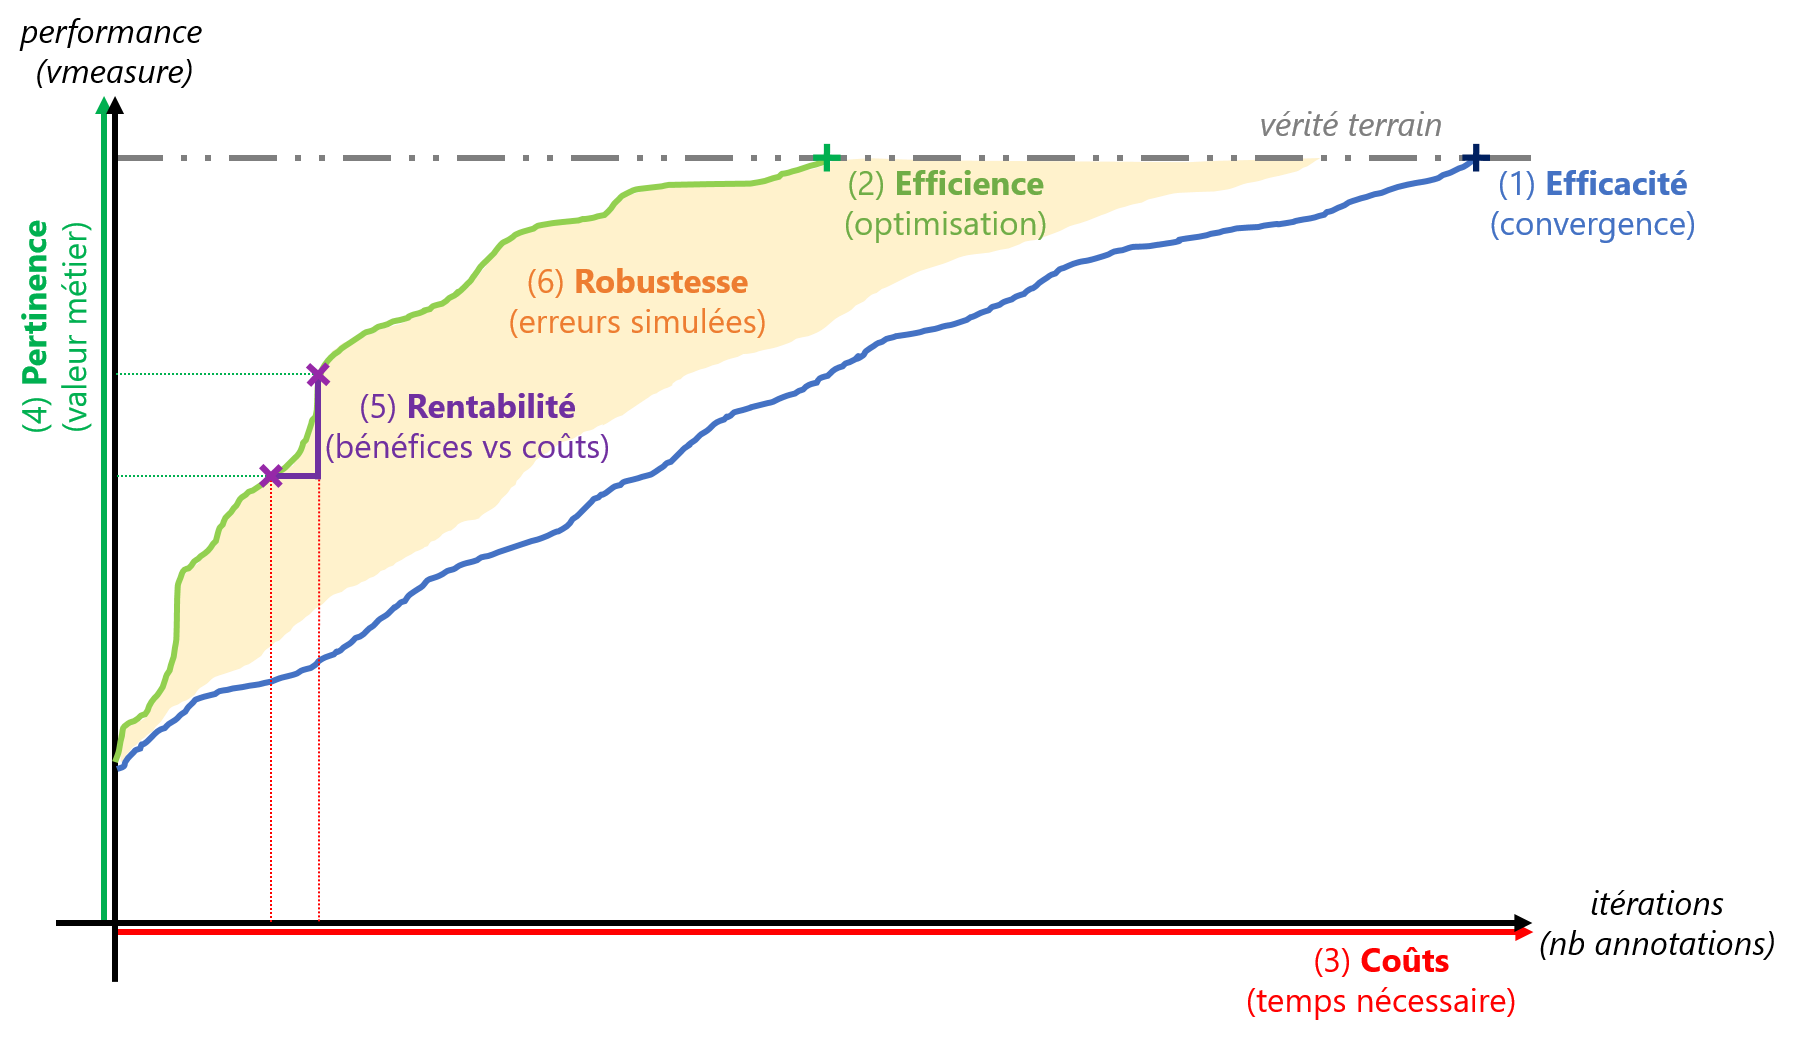
\includegraphics[width=0.95\textwidth]{figures/hypotheses-06-robustesse}
			\caption{
				Illustration des études réalisées sur le \textit{clustering} interactif (\textit{étape 6/6}) en schématisant l'évolution de la pertinence (\textit{valeur métier évaluée par l'expert et exprimé en nombre de clusters}) d'une base d'apprentissage en cours de construction en fonction du coût temporel de la méthode (\textit{temps nécessaire à l'expert métier et à la machine}), ainsi que les marges d'erreurs représentant l'impact de différences d'annotation sur le nombre d'itérations nécessaire à la méthode.
			}
			\label{figure:4.6-HYPOTHESE-ROBUSTESSE}
		\end{figure}
	\end{tcolorbox}
		
	% Résumé de l'étude.
	Afin de vérifier cette hypothèse, nous organisons trois expériences :
	\begin{itemize}
		\item une étude de cas sur la \textbf{correction des incohérences d'annotation} (cf. \textsc{Section~\ref{section:4.6.1-ETUDE-ROBUSTESSE-INTERET-CORRECTION-INCOHERENCES}}) ;
		\item une simulation de l'\textbf{impact des différences d'annotation} sur les résultats de la méthode (cf. \textsc{Section~\ref{section:4.6.2-ETUDE-ROBUSTESSE-SIMULATION-IMPACT-DIFFERENCES}}) ;
		\item une étude de cas sur le \textbf{score inter-annotateurs} obtenu lors d'une annotation de contraintes en situation réelle avec plusieurs opérateurs (cf. \textsc{Section~\ref{section:4.6.3-ETUDE-ROBUSTESSE-SCORE-INTER-ANNOTATEURS}}).
	\end{itemize}
	
	
	%%%
	%%% Subsection 4.6.1: Étude de l'intérêt de la correction des incohérences d'annotation.
	%%%
	\subsection{Étude de l'intérêt de la correction des incohérences d'annotation}
	\label{section:4.6.1-ETUDE-ROBUSTESSE-INTERET-CORRECTION-INCOHERENCES}
		
		% Objectif de l'expérience.
		Nous cherchons à estimer la robustesse du \textit{clustering} interactif face aux incohérences d'annotation.
		Dans cette étude, nous nous intéressons plus particulièrement à l'intérêt de la détection et de la correction des conflits présents dans les contraintes.
		En effet, deux approches de travail s'opposent :
		\begin{itemize}
			\item une approche \textit{naïve} ignorant simplement les conflits : celle-ci n'engendre pas de coûts supplémentaires, mais elle s'expose aux risques de dérives de fonctionnement ;
			\item une seconde approche \textit{avec correction} des conflits : celle-ci nécessite de revoir ou de ré-annoter des contraintes, impliquant un coût supplémentaire, mais permet de limiter l'impact de dérives potentielles.
		\end{itemize}
		Pour trancher entre ces deux options, nous simulons ces deux approches afin d'estimer si l'absence de correction induit une différence significative de notre méthode d'annotation.
	
		%%% Protocole expérimental.
		\subsubsection{Protocole expérimental}
			
			% Pseudo-code.
			Pour résumer le protocole expérimental que nous décrivons ci-dessous, vous pouvez vous référer au pseudo-code décrit dans \textsc{Algorithme~\ref{algorithm:4.6.1-ETUDE-ROBUSTESSE-INTERET-CORRECTION-INCOHERENCES-PROTOCOLE}}.
			
			\begin{algorithm}
				\KwData{jeu de données annotées (vérité terrain)}
				\KwIn{liste de taux de différences à insérer, stratégies de correction de conflits}
				%
				\ForEach{stratégie de correction et taux de différences à insérer}{
					\textbf{initialisation (données)}: récupérer les données et la vérité terrain \;
					\textbf{initialisation (contraintes)}: créer une liste vide de contraintes \;
					\textbf{prétraitement}: supprimer le bruit dans les données avec \texttt{prep.simple} \;
					\textbf{vectorisation}: transformer les données en vecteurs avec \texttt{vect.tfidf} \;
					\textbf{clustering initial}: regrouper les données par similarité avec \texttt{clust.kmeans.cop} \;
					\textbf{évaluation}: estimer l'équivalence entre le \textit{clustering} et la vérité terrain \;
					\Repeat{annotation de toutes les contraintes possibles}{
						\textbf{échantillonnage}: sélectionner des contraintes avec \texttt{samp.closest.diff} \;
						\textbf{choix des incohérences}: définir les contraintes erronées \;
						\textbf{simulation d'annotation}: déterminer les contraintes avec la vérité terrain \;
						\If{stratégie de correction naïve}{
							\textbf{intégration naïve}: ajouter les nouvelles contraintes au gestionnaire de contraintes, et ignorer les conflits avec le gestionnaire de contraintes \;
						}
						\ElseIf{stratégie avec correction}{
							\textbf{intégration corrective}: ajouter les nouvelles contraintes au gestionnaire de contraintes, et ré-annoter les annotations en conflit \;
						}
						\textbf{clustering}: regrouper les données par similarité avec \texttt{clust.kmeans.cop} \;
						\textbf{évaluation}: estimer l'équivalence entre le \textit{clustering} et la vérité terrain \;
					}
					\textbf{analyse locale}: afficher l'évolution de la performance par rapport à la vérité terrain en fonction du nombre de contraintes \;
				}
				\textbf{analyse}: déterminer l'impact des stratégies de correction en fonction des taux de différences insérées \;
				%
				\KwResult{discussion sur l'intérêt de la correction des incohérences}
				%
				\caption{\textit{
					Description en pseudo-code du protocole expérimental de l'étude d'intérêt de la correction des incohérences d'annotation.
				}}
				\label{algorithm:4.6.1-ETUDE-ROBUSTESSE-INTERET-CORRECTION-INCOHERENCES-PROTOCOLE}
			\end{algorithm}
			
			% Description de la vérité terrain.
			Nous utilisons comme vérité terrain le jeu de données \texttt{Bank Cards (v1.0.0)} : ce dernier traite des demandes les plus fréquentes des clients en ce qui concerne la gestion de leur carte bancaire.
			Il est composé de $500$ questions rédigées en français et réparties en $10$ classes (\texttt{perte ou vol de carte}, \texttt{carte avalée}, \texttt{commande de carte}, ...).
			Pour plus de détails, consultez l'annexe~\ref{annex:A.1-DATASET-BANK-CARDS}.
			
			% Description des tentatives de la méthode avec simulation d'erreurs.
			Sur ce jeu de données, nous exécutons une tentative complète\footnote{
				Tentative complète : itérations d'échantillonnage, d'annotation et de \textit{clustering} jusqu'à annotation de toutes les contraintes possibles.
			}
			de la méthode du \textit{clustering} interactif en utilisant notre paramétrage favori (voir \textsc{Section~\ref{section:4.3-HYPOTHESE-COUTS}}).
			Toutefois, contrairement aux précédents expériences, nous allons ajouter un pourcentage de contraintes divergentes à chaque itération :
			\begin{itemize}
				\item Le taux de différences insérées, variant de $0$\% à $50$\% par pas de $5$\%, reste fixe tout au long d'une même tentative de notre méthode : nous pouvons ainsi analyser l'impact d'un taux de différences fixe sur les résultats au courant des itérations ;
				\item Les contraintes divergentes à insérer sont tirées aléatoirement parmi le lot de contraintes qui aurait été échantillonné au cours d'une tentative sans introduction de différences : ainsi, nous pouvons comparer itération par itération toutes ces simulations car elles partagent la même base de contraintes (aux valeurs de \texttt{MUST-LINK} et \texttt{CANNOT-LINK} près) ;
			\end{itemize}
			
			% Description des tentatives de la méthode avec gestion des conflits.
			Puisque nous introduisons des différences d'annotations, des conflits peuvent apparaître dans le gestionnaire de contraintes.
			Pour rappel, un conflit est détecté dans le cas où l'ajout d'une nouvelle contrainte annotée contredit ce qui a été précédemment déduit grâce aux propriétés de transitivité des contraintes de types \texttt{MUST-LINK}et \texttt{CANNOT-LINK} (voir \textsc{Figure~\ref{figure:3.3-CONTRAINTES-TRANSITIVITE}} en \textsc{Section~\ref{section:3.3.2-GESTION-DES-CONTRAINTES}}).
			Pour les traiter, nous testons deux approches :
			\begin{itemize}
				\item l'approche \textit{naïve} ignorant simplement les conflits : si la prochaine contrainte à ajouter est incompatible avec la base de contraintes déjà intégrées au gestionnaire, alors nous ignorons simplement son existence sans remettre en question les précédentes annotations ;
				\item l'approche \textit{avec correction} des conflits : pour simuler la correction d'un expert, nous recréons à chaque itération le gestionnaire de contraintes en intégrant d'abord les contraintes correctes puis les contraintes divergentes ; ainsi, les conflits ne peuvent arriver qu'à l'ajout d'une contrainte divergente, et il suffit d'ajouter sa version exacte pour simuler la correction de l'expert.
			\end{itemize}
			
			% Description des tentatives de la méthode avec les répétitions.
			Ainsi, il y a donc $11$ taux de différences, chacun suivant $2$ approches de gestion de conflits, et chacune de ces simulations d'incohérences seront répétées $10$ fois sur chaque tentative complète de la méthode pour contrer les aléas statistiques des tirages de contraintes divergentes, ce qui représente $220$ simulations par tentatives.
			Enfin, chaque tentative complète de \textit{clustering} interactif est répétée $5$ fois pour contrer les aléas statistiques des exécutions, ce qui représente un total de $1100$ tentatives complètes à simuler.

			% Description de l'analyse.
			Enfin, nous affichons l'évolution de la performance moyenne du \textit{clustering} obtenu en fonction des divers taux de différences simulées, et discutons de l'impact au cours des itérations de la présence ou de l'absence de corrections des conflits d'annotations détectés.
			
			% Référence scripts.
			\begin{leftBarInformation}
				Les scripts de l'expérience, réalisés avec des \textit{notebooks} Python (\cite{van-rossum-drake:2009:python-reference-manual}), sont disponibles dans un dossier dédié de~\cite{schild:2021:cognitivefactory-interactiveclusteringcomparativestudy}.
			\end{leftBarInformation}

		%%% Résultats
		\subsubsection{Résultats obtenus}
		
			% Description statistiques.
			La \textsc{Figure~\ref{figure:4.6.1-ETUDE-ROBUSTESSE-INTERET-CORRECTION-INCOHERENCES}} représente l'évolution moyenne de la \texttt{v-measure} du \textit{clustering} en fonction du nombre de contraintes annotées au cours des itérations de la méthode, et cette évolution est déclinée pour les $11$ taux de différences simulés et les $2$ approches de gestion des conflits.
			Les contraintes utilisées sont basées sur les échantillonnages réalisées au cours des tentatives n'introduisant pas de différences d'annotation par rapport à la vérité terrain : comme les mêmes contraintes sont donc utilisées (aux valeurs d'annotations près), toutes les courbes sont comparables point par point.
			
			% Warning : Troncage à 3000.
			\begin{leftBarWarning}
				Toutefois, il est important de noter que les tentatives sans contraintes ont besoin de maximum $3~000$ contraintes pour annoter toutes les contraintes possibles et leurs transitivités (moyenne: $2~488$, écart-type: $327$).
				Au delà de cette limite, il faudrait échantillonner de nouvelles contraintes pour les tentatives divergentes, mais les bases de contraintes utilisées ne seraient alors plus comparables.
				Nous décidons donc de tronquer les différentes courbes à $3~000$ contraintes, qu'il y eut convergence ou non, et nous analysons ces résultats partiels.
			\end{leftBarWarning}
			
			% Figure.
			\begin{figure}[!htb]
				\centering
				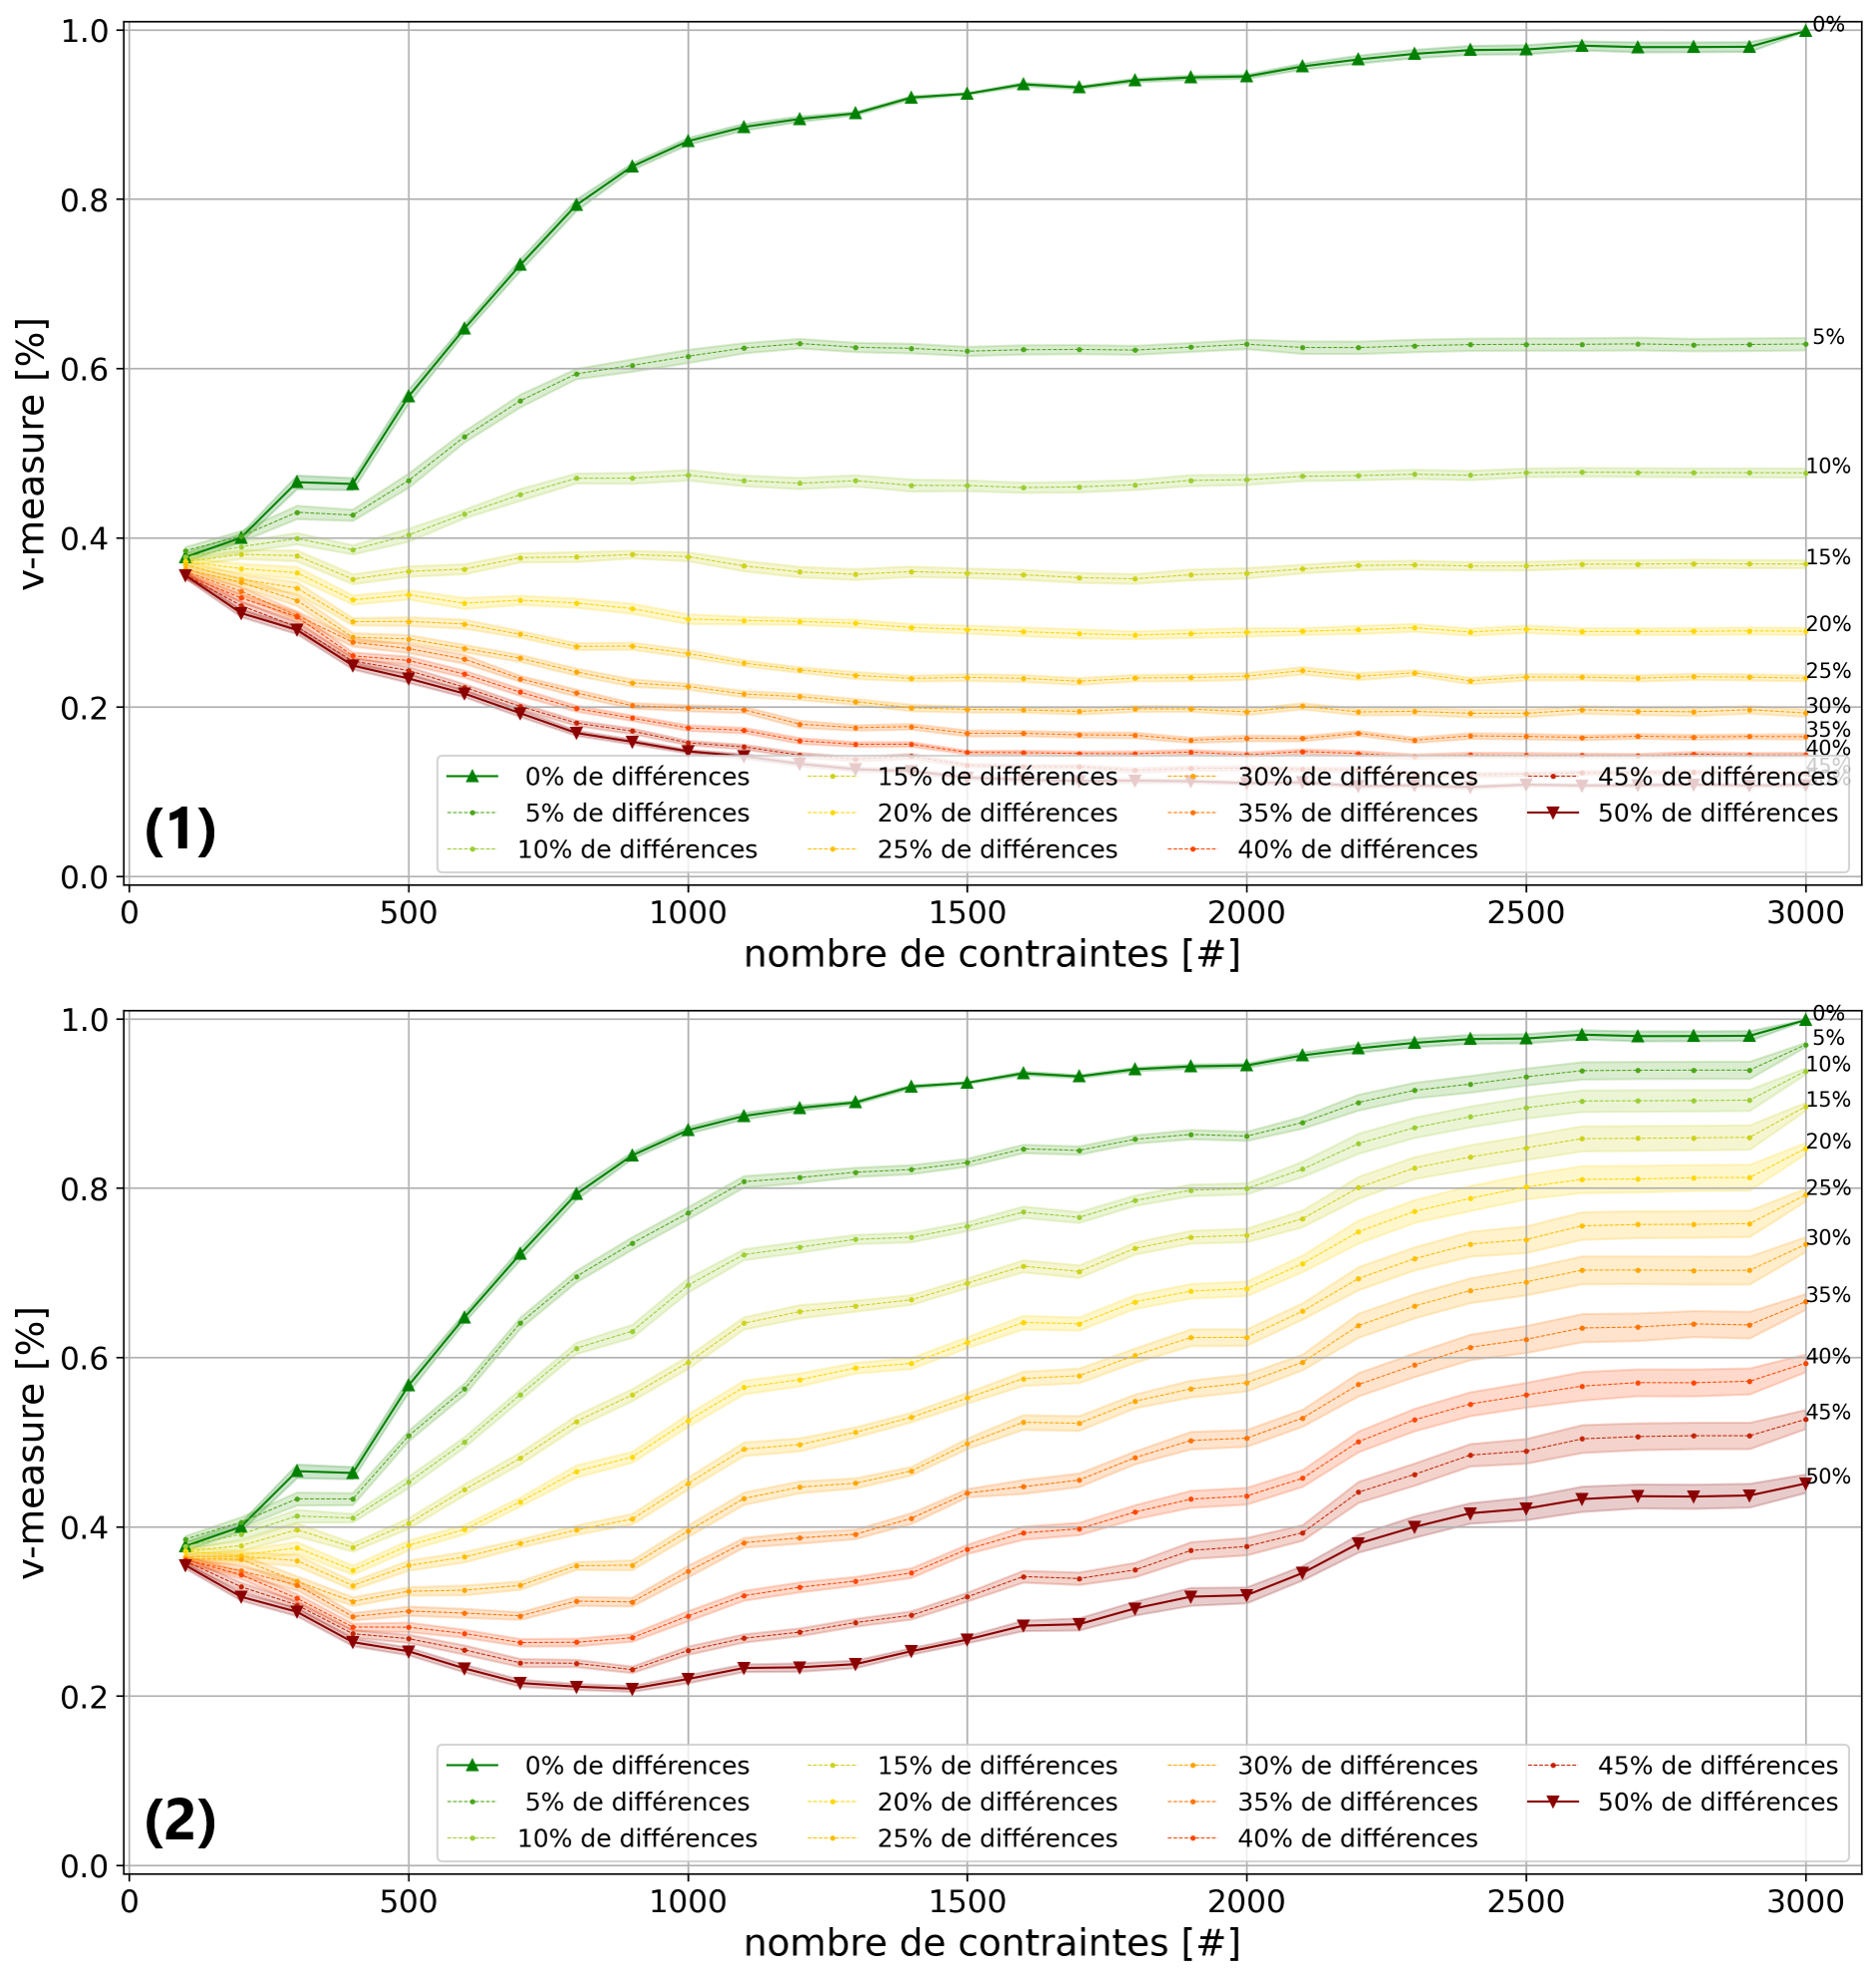
\includegraphics[width=0.95\textwidth]{figures/etude-erreur-interet-correction-closest}
				\caption{
					Évolution des similitudes moyennes (calculées en terme de \texttt{v-measure}) des résultats de \textit{clustering} des tentatives introduisant des incohérences d'annotation par rapport à la vérité terrain au cours des itérations.
					Les dégradés de couleurs des courbes représentent les déclinaisons de ces évolutions en fonction des différents taux d'annotations erronées (allant de $0$\% et $50$\%).
					\textbf{(1)} représente l'approche naïve ignorant les conflits d'annotation
					et \textbf{(2)} représente l'approche corrigeant les conflits détectés par le gestionnaire de contraintes.
					Toutes les courbes sont tronquées à $3~000$ contraintes (nombre maximum de contraintes nécessaire à une tentatives sans incohérence pour converger vers la vérité terrain).
				}
				\label{figure:4.6.1-ETUDE-ROBUSTESSE-INTERET-CORRECTION-INCOHERENCES}
			\end{figure}
			
			% Description de la figure: cas naïf.
			Tout d'abord, observons l'approche \textit{naïve}, ignorant simplement les conflits (voir \textsc{Figure~\ref{figure:4.6.1-ETUDE-ROBUSTESSE-INTERET-CORRECTION-INCOHERENCES}} \textbf{(1)}).
			Nous pouvons constater que les performances (basées sur la vérité terrain) plafonnent très rapidement si des incohérences sont introduites : dès $5$\% de différences, le score de \texttt{v-measure} stagne autour de $65$\% à partir de $1~000$ contraintes, alors qu'une performance théorique d'environ $90$\% serait attendue pour une tentative n'ayant pas de différences d'annotation.
			D'autre part, si le taux de contraintes divergentes introduites est supérieur à $15$\%, nous pouvons remarquer que ces performances diminuent avant de stagner à des valeurs inférieures à $40$\% de \texttt{v-measure}.
			Pour finir sur cette première approche, tout porte à croire que ces faibles seuils performances perdurent au delà des $3~000$ contraintes (figure tronquée) : les tentatives s'éloignent donc significativement de la vérité terrain si des incohérences d'annotation sont insérées.
			
			
			% Description de la figure: cas correctif.
			Observons désormais l'approche \textit{avec correction}, ré-évaluant les contraintes lorsqu'un conflit est détecté par le gestionnaire de contraintes (voir \textsc{Figure~\ref{figure:4.6.1-ETUDE-ROBUSTESSE-INTERET-CORRECTION-INCOHERENCES}} \textbf{(2)}).
			Nous pouvons constater que les tentatives introduisant des contraintes divergentes subissent aussi un retard de performances, mais aucun plateau de performance n'apparaît.
			Pour les tentatives possédant au moins $25$\% d'incohérences, des régressions de performances apparaissent sur les premières itérations, mais toutes les courbes sont à nouveau croissantes au delà d'un nombre de $1~000$ contraintes.
			Pour conclure sur cette seconde figure, on observe une convergence générale vers la vérité terrain bien que celle-ci soit ralentie, et on peut espérer que cette convergence se poursuit au delà des $3~000$ contraintes (figure tronquée).

		%%% Discussion
		\subsubsection{Discussion}
		
			% Rappel de l'objectif : Intérêt de la correction en cas d'incohérences.
			L'objectif de cette étude consiste à montrer l'intérêt de la correction en cas de conflits dans les contraintes annotées.
			Pour cela, nous avons comparé deux approches : une approche naïve ignorant simplement les conflits, et une deuxième approche les corrigeant si ces derniers sont détectés par le mécanisme de gestion des contraintes.
		
			% Analyse : Super important de corriger !
			D'après l'analyse de la \textsc{Figure~\ref{figure:4.6.1-ETUDE-ROBUSTESSE-INTERET-CORRECTION-INCOHERENCES}}, nous pouvons clairement déduire que l'absence de correction des incohérences pénalise la méthode et entraîne une dérive significative des résultats.
			En effet, sur le jeu de données utilisé comme vérité terrain, nous constatons une perte irréversible d'au moins $35$\% de \texttt{v-measure} dès l'introduction de $5$\% d'incohérences d'annotation, pénalisant ainsi sérieusement les performances de la méthode.
			Toutefois, la mise en oeuvre d'un mécanisme simple de correction semble estomper en partie ces régressions de performances et permettre à certaines tentatives introduisant des erreurs de rester néanmoins compétitives
			(\textit{par exemple : les expériences introduisant $25$\% d'erreurs peuvent espérer atteindre $80$\% de \texttt{v-measure} en corrigeant leurs incohérences, alors que l'approche naïve les condamnait à un \texttt{v-measure} moyenne inférieure à $30$\%}).
			Nous pouvons donc assurément conclure sur la nécessité de vérifier sa base de contraintes et de corriger toute incohérences s'y trouvant.
			
			% Remarque : Idées pour améliorer la détection et la correction.
			Une telle conclusion confirme la sensibilité aux erreurs de cette approche incrémentale : si une erreur apparaît, elle peut rapidement se propager et impacter les résultats de la méthode.
			Dans notre cas, nous avons optimisé l'implémentation de notre \textit{clustering} interactif pour obtenir un corpus d'apprentissage pertinent en un minimum d'annotation de contraintes.
			Or obtenir un nombre minimal implique de limiter la redondance parmi les contraintes annotées.
			De ce fait, certaines incohérences mal placées peuvent fortement influencer la base de contraintes et ainsi faire diverger les résultats.
			Pour contrer ce problème, nous avons deux pistes pouvant être explorées :
			\begin{itemize}
				% Introduction de redondance d'annotation.
				\item concevoir une nouvelle méthode d'échantillonnage introduisant intentionnellement des redondances dans la base de contraintes annotées : ce moyen compte alors sur les propriétés de transitivité du graphe de contraintes pour identifier d'éventuelles incohérences d'annotation isolée ou masquée.
				Cette piste a cependant le désavantage d'ajouter de nouvelles contraintes peu informative dans le simple but de mieux détecter certaines incohérences, introduisant donc un coût supplémentaire : il y a donc un choix à faire entre la qualité du résultat et la rapidité de son obtention ;
				% Confronter la vision des annotateurs.
				\item confronter la vision des annotateurs sur les mêmes contraintes : en faisant annoter les contraintes par deux opérateurs différents, les incohérences ou divergences d'annotation peuvent être révélées ; en ajoutant un troisième, nous pouvons organiser sereinement les débats pour corriger ces incohérences et décider des adaptations éventuelles à prévoir dans le guide d'annotation.
				Une telle approche ajoute bien entendu un coût supplémentaire (plusieurs annotateurs), mais elle a néanmoins l'avantage de recentrer les discussions des revues d'annotation sur les différences entre cas d'usage métier (\textit{compétences métiers}) plutôt que sur les différences entre représentations abstraites du problème à modéliser (\textit{compétences analytiques}).
			\end{itemize}
			
			% Discussions et ouverture
			\begin{leftBarAuthorOpinion}
				% Une différence n'est pas forcément une erreur.
				Ce dernier point permet d'ouvrir une discussion intéressante sur les raisons de ces incohérences d'annotations.
				Les cas les plus évidents sont ceux des erreurs d’inattentions, mais de telles différences sont facilement identifiables et corrigeables par un mécanisme de redondance (\textit{en vérifiant la transitivité des contraintes ou en ajoutant d'autres annotateurs sur un même lot d'annotation}).
				
				% Cas plus complexe de la subjectivité.
				En revanche, un cas plus complexe concerne la subjectivité des opérateurs :
				en effet, les annotations divergentes ne sont pas forcément des "\textit{erreurs}", elles peuvent aussi représenter une différence de vision de l'expert métier, conduisant pas-à-pas vers une \textbf{autre} vérité terrain (celle-ci est pertinente de \textbf{son} point de vue).
				On peut prendre l'exemple de la simulation introduisant $50$\% d'incohérences : cela exprime que deux opérateurs sont constamment en désaccord, il est donc normal que les résultats divergent autant...
				
				% S'intéresser à l'estimation de cette divergence.
				Ainsi, bien que la labellisation par contraintes semble plus simple et moins coûteuse à réaliser pour un expert métier, des différences d'opinions pourront toujours être constatées parmi plusieurs experts, et il est important d'organiser des sessions de confrontation pour harmoniser les points de vue (voir \textsc{Section~\ref{section:2.3.3-DEFIS-ANNOTATION-ASPECT-HUMAIN}}).
				Dans la suite de cette étude, nous nous intéressons à l'estimation de l'impact des divergences entre deux annotateurs sans mécanisme de redondance d'annotation.
			\end{leftBarAuthorOpinion}
	
	
	%%%
	%%% Subsection 4.6.2: Étude de l'impact des incohérences d'annotation sur les résultats.
	%%%
	\subsection{Étude de l'impact des incohérences d'annotation sur les résultats}
	\label{section:4.6.2-ETUDE-ROBUSTESSE-SIMULATION-IMPACT-DIFFERENCES}
		
		% Objectif de l'expérience.
		Dans la section précédente, nous avons montré l'intérêt de corriger les incohérences dans les annotations, mais aussi la nécessité d'employer plusieurs opérateurs pour confronter les points de vue et ainsi mettre plus facilement en évidence les contraintes divergentes.
		Dans cette étude, nous nous intéressons plus particulièrement à l'impact d'une différence d'annotation et son impact sur l'écart de similitude par rapport à la vérité terrain.
		Nous réalisons cette analyse sur des jeux de données de différentes tailles et pour plusieurs taux d'incohérences insérées.
		
		% Note de l'auteur : chercher la différence plutôt que le retard.
		\begin{leftBarAuthorOpinion}
			
			% Ancien objectif.
			Initialement, nous voulions estimer le retard (en terme de nombre de contraintes) engendré par l'introduction d'un certain taux d'incohérences dans les annotations pour atteindre un objectif de $90$\% de \texttt{v-measure} par rapport à la vérité terrain (objectif d'annotation partielle).
			Cependant, un tel objectif n'était pas atteignable : en effet, nous avons vu dans la \textsc{Section~\ref{section:4.6.1-ETUDE-ROBUSTESSE-INTERET-CORRECTION-INCOHERENCES}} que l'introduction de d'incohérences fait diverger le \textit{clustering} vers une autre vérité terrain.
			Ainsi, sans mécanisme de redondance ni doubles annotations, il est possible que le score de \texttt{v-measure} obtenu reste inférieur au seuil d'analyse que nous nous aurions fixé.
			Par exemple, en regardant la \textsc{Figure~\ref{figure:4.6.2-ETUDE-ROBUSTESSE-SIMULATION-IMPACT-DIFFERENCES}}, nous pouvons supposer que les tentatives ayant $50$\% d'incohérences ne dépasseront jamais le score de $90$\% de \texttt{v-measure}...
			
			% Nouvel objectif.
			Nous avons donc adapté l'objectif de cette étude : au lieu d'estimer le retard en nombre de contraintes pour atteindre $90$\% de \texttt{v-measure}, nous allons estimer l'écart de \texttt{v-measure} des tentatives introduisant des incohérences pour un nombre de contraintes donné.
			Pour cette analyse, nous fixons le nombre de contraintes à celui nécessaire pour obtenir une moyenne de $90$\% de \texttt{v-measure} avec des tentatives n'introduisant pas d'incohérences.
			La figure \textsc{Figure~\ref{figure:4.6.2-ETUDE-ROBUSTESSE-SIMULATION-IMPACT-DIFFERENCES}} illustre le problème et le choix de faire une étude pour un nombre de contrainte fixé.
			
			% Schéma.
			\begin{figure}[H]
				\centering
				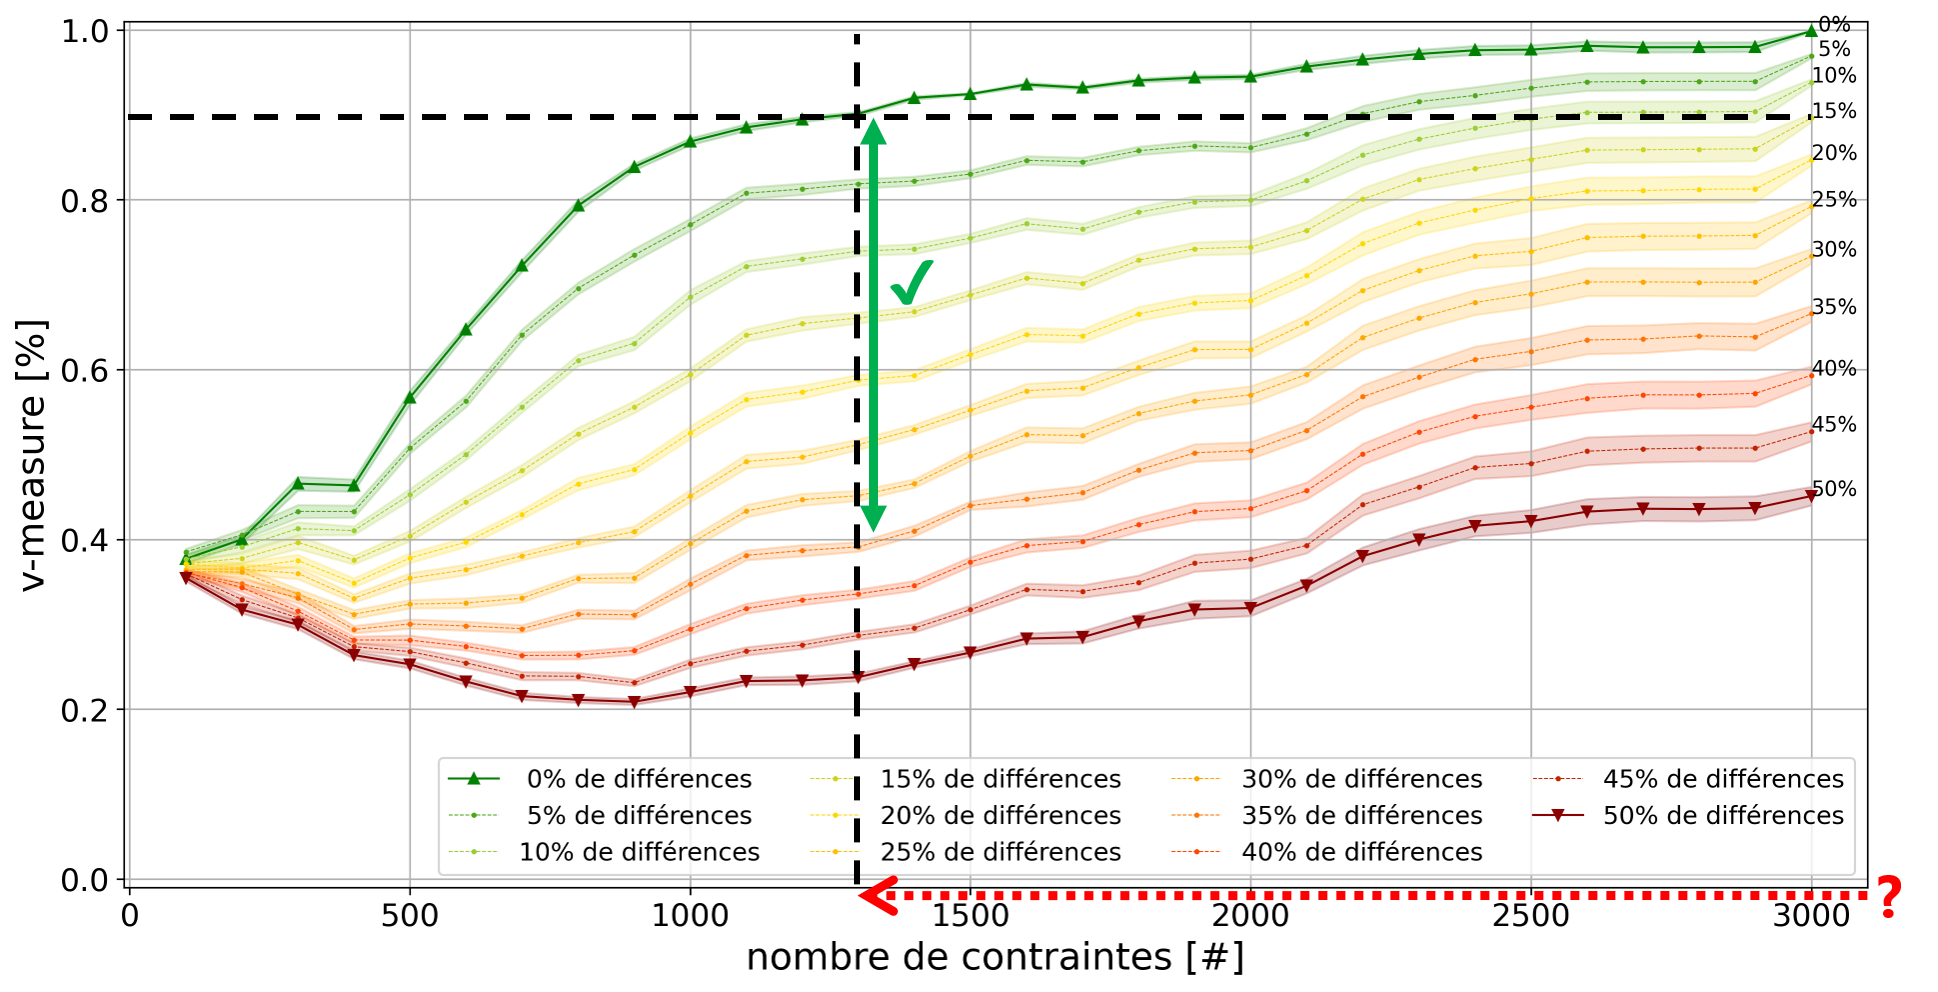
\includegraphics[width=0.80\textwidth]{figures/etude-erreur-simulation-impact-schema}
				\caption{
					Schéma illustrant l'impossibilité d'estimer le retard engendré l'introduction d'erreur (voir les barres en pointillées rouges) mais la possibilité d'estimer l'écart de similitude pour un nombre de contraintes données (voir la barre continue verte).
				}
				\label{figure:4.6.2-ETUDE-ROBUSTESSE-SIMULATION-IMPACT-DIFFERENCES}
			\end{figure}
		\end{leftBarAuthorOpinion}
	
		%%% Protocole expérimental.
		\subsubsection{Protocole expérimental}
			
			% Pseudo-code.
			Pour résumer le protocole expérimental que nous décrivons ci-dessous, vous pouvez vous référer au pseudo-code décrit dans \textsc{Algorithme~\ref{algorithm:4.6.2-ETUDE-ROBUSTESSE-SIMULATION-IMPACT-DIFFERENCES-PROTOCOLE}}.
			
			\begin{algorithm}
				\KwData{jeux de données annotées (vérités terrains) de tailles différentes}
				\KwIn{liste de taux de différences à insérer}
				%
				\ForEach{jeux de données à tester et taux de différences à insérer}{
					\textbf{initialisation (données)}: récupérer les données et la vérité terrain \;
					\textbf{initialisation (contraintes)}: créer une liste vide de contraintes \;
					\textbf{prétraitement}: supprimer le bruit dans les données avec \texttt{prep.simple} \;
					\textbf{vectorisation}: transformer les données en vecteurs avec \texttt{vect.tfidf} \;
					\textbf{clustering initial}: regrouper les données par similarité avec \texttt{clust.kmeans.cop} \;
					\textbf{évaluation}: estimer l'équivalence entre le \textit{clustering} et la vérité terrain \;
					\Repeat{annotation de toutes les contraintes possibles}{
						\textbf{échantillonnage}: sélectionner des contraintes avec \texttt{samp.closest.diff} \;
						\textbf{choix des incohérences}: définir les contraintes erronées \;
						\textbf{simulation d'annotation}: déterminer les contraintes avec la vérité terrain \;
						\textbf{intégration corrective}: ajouter les nouvelles contraintes au gestionnaire de contraintes, et ré-annoter les annotations en conflit \;
						\textbf{clustering}: regrouper les données par similarité avec \texttt{clust.kmeans.cop} \;
						\textbf{évaluation}: estimer l'équivalence entre le \textit{clustering} et la vérité terrain \;
					}
					\textbf{analyse locale}: identifier le nombre moyen de contraintes nécessaires à une tentative n'introduisant pas d'incohérence pour atteindre $90$\% de \texttt{v-measure}, et noter le score de \texttt{v-measure} obtenu par de la tentative courante pour le nombre de contraintes identifié \;
				}
				\textbf{analyse générale}: déterminer l'impact des incohérences par taux de différences et par taille de jeux de données \;
				%
				\KwResult{discussion sur l'impact des incohérences sur le \textit{clustering} obtenu}
				%
				\caption{\textit{
					Description en pseudo-code du protocole expérimental de l'impact des incohérences d'annotation sur les résultats.
				}}
				\label{algorithm:4.6.2-ETUDE-ROBUSTESSE-SIMULATION-IMPACT-DIFFERENCES-PROTOCOLE}
			\end{algorithm}
			
			% Détails de l'expérience.
			Nous reprenons dans les grandes lignes le protocole expérimental de la précédente étude sur l'intérêt de la correction des incohérences d'annotation (voir \textsc{Section~\ref{section:4.6.1-ETUDE-ROBUSTESSE-INTERET-CORRECTION-INCOHERENCES}}.
			
			% Description des jeux de données.
			Nous utilisons cette fois deux vérités terrains comme références :
			\begin{itemize}
				\item le jeu de données \texttt{Bank Cards (v2.0.0)} : ce dernier traite des demandes les plus fréquentes des clients en ce qui concerne la gestion de leur carte bancaire. Il est composé de $1~000$ questions rédigées en français et réparties en $10$ classes (\texttt{perte ou vol de carte}, \texttt{carte avalée}, \texttt{commande de carte}, ...). Pour plus de détails, consultez l'annexe~\ref{annex:A.1-DATASET-BANK-CARDS} ;
				\item le jeu de données \texttt{MLSUM FR Train Subset (v1.0.0-schild)} : ce dernier concerne les titres d'articles de journaux issus des catégories de publication les plus communes. Il est composé de $744$  titres d'articles rédigés et répartis en $14$ classes (\textit{économie}, \textit{sport}, ...). Pour plus de détails, consultez l'annexe~\ref{annex:A.2-DATASET-MLSUM-SUBSET-SCHILD} ;
			\end{itemize}
			
			Pour utiliser facilement plusieurs jeux de données de tailles différentes tout en maîtrisant leur contenu, nous avons donc dupliqué aléatoirement des données issues de ces jeux de référence en y insérant des fautes de frappes.
			La taille des jeux de données générés varie entre $1~000$ à $5~000$ par pas de $500$.
			Il y a donc $9$ variations de chaque jeu de références, soit $18$ jeux utilisés de tailles différentes.
			
			% Remarque.
			\begin{leftBarWarning}
				Dans le cadre de cette étude, nous faisons l'hypothèse que cette création artificielle de données n'a pas d'impact majeur sur le nombre de contraintes nécessaires pour converger vers une vérité terrain.
			\end{leftBarWarning}
			
			% Description des tentatives de la méthode avec simulation d'erreurs.
			Sur ces jeux de données, nous exécutons une tentative complète\footnote{
				Tentative complète : itérations d'échantillonnage, d'annotation et de \textit{clustering} jusqu'à annotation de toutes les contraintes possibles.
			}
			de la méthode du \textit{clustering} interactif en utilisant notre paramétrage favori (voir \textsc{Section~\ref{section:4.3-HYPOTHESE-COUTS}}).
			A nouveau, nous allons ajouter un pourcentage de contraintes divergentes à chaque itération :
			\begin{itemize}
				\item Le taux de différences insérées, variant de $0$\% à $25$\% par pas de $5$\%, reste fixe tout au long d'une même tentative de notre méthode : nous pouvons ainsi analyser l'impact d'un taux de différences fixe sur les résultats au courant des itérations ;
				\item Les contraintes divergentes à insérer sont tirées aléatoirement parmi le lot de contraintes qui aurait été échantillonné au cours d'une tentative sans introduction de différences : ainsi, nous pouvons comparer itération par itération toutes ces simulations car elles partagent la même base de contraintes (aux valeurs de \texttt{MUST-LINK} et \texttt{CANNOT-LINK} près) ;
			\end{itemize}
			
			% Description des tentatives de la méthode avec gestion des conflits.
			Puisque nous introduisons des différences d'annotations, des conflits peuvent apparaître dans le gestionnaire de contraintes.
			Pour rappel, un conflit est détecté dans le cas où l'ajout d'une nouvelle contrainte annotée contredit ce qui a été précédemment déduit grâce aux propriétés de transitivité des contraintes de types \texttt{MUST-LINK}et \texttt{CANNOT-LINK} (voir \textsc{Figure~\ref{figure:3.3-CONTRAINTES-TRANSITIVITE}} en \textsc{Section~\ref{section:3.3.2-GESTION-DES-CONTRAINTES}}).
			En tirant parti des conclusion de la précédente étude, nous choisissons de corriger ces incohérences dès leur détection.
			Pour simuler cette correction de l'expert, nous recréons à chaque itération le gestionnaire de contraintes en intégrant d'abord les contraintes correctes puis les contraintes divergentes ; ainsi, les conflits ne peuvent arriver qu'à l'ajout d'une contrainte divergente, et il suffit d'ajouter sa version exacte pour simuler la correction de l'expert.
			
			% Description des tentatives de la méthode avec les répétitions.
			Ainsi, il y a donc $6$ taux de différences, et chacune de ces simulations d'incohérences seront répétées $2$ fois sur chaque tentative complète de la méthode pour limiter au mieux les aléas statistiques des tirages de contraintes divergentes, ce qui représente $12$ simulations par tentatives.
			Enfin, chaque tentative complète de \textit{clustering} interactif est répétée $2$ fois pour limiter au mieux les aléas statistiques des exécutions, soit un nombre de $24$ tentatives complètes par jeu de données, ce qui représente un total de $432$ tentatives à simuler au cours de cette expérience.
			
			% Description de l'analyse.
			Enfin, dans l'optique de réaliser l'analyse de l'écart de performances engendré par l'introduction de différences d'annotation, nous procédons en trois temps :
			\begin{itemize}
				% Estimer le nombre de contraintes.
				\item nous estimons d'abord, pour chaque taille de jeu de données, le nombre moyen de contraintes nécessaires à une tentative n'introduisant pas d'incohérence pour atteindre un score de $90$\% de \texttt{v-measure} par rapport à sa vérité terrain ;
				% Retenir la vmeasure pour ce nombre de contraintes.
				\item nous estimons ensuite, pour chaque tentatives introduisant des incohérences, son score de \texttt{v-measure} par rapport sa version n'introduisant pas de contraintes et pour le nombre de contraintes déterminé précédemment (celui nécessaire à la tentative n'introduisant pas d'incohérence pour atteindre un score de $90$\%) ;
				% Comparer l'écart.
				\item enfin, nous discutons de ces scores moyens pour les différentes tailles de jeu de données et les différents taux d'incohérences introduites.
			\end{itemize}
			La \textsc{Figure~\ref{figure:4.6.2-ETUDE-ROBUSTESSE-SIMULATION-IMPACT-DIFFERENCES}} illustre cette analyse pour un nombre de contraintes fixé.
			
			% Note de l'auteur sur le choix du nombre de contraintes.
			\begin{leftBarAuthorOpinion}
				Il est à noter que nous aurions pu estimer ce nombre de contraintes grâce à l'\textsc{Équation~\ref{equation:4.3.3-ETUDE-COUT-NOMBRE-CONTRAINTES}} ($3.15 \cdot \texttt{dataset\_size}$), mais comme cette estimation théorique est une moyenne.
				Nous avons préféré mesurer directement le nombre exact de contraintes nécessaires pour chaque tentative afin de ne pas avoir à calculer le score de \texttt{v-measure} moyen moyenne sur la base d'une estimation théorique moyenne du nombre de contraintes.
			\end{leftBarAuthorOpinion}
			
			% Remarque sur le faible nombre de redondances des tentatives.
			\begin{leftBarWarning}
				Ces simulations étant plus lourdes que les précédentes, en considérant le manque de temps pour réaliser cette étude, nous avons du diminuer le nombre de répétitions de nos tentatives ($1$ pour le génération des jeux de données, $2$ pour l'insertion des incohérences, $2$ pour l’exécution des tentatives complètes de la méthode).
				Les résultats obtenus nous permettent tout de même de discuter des tendances générales, mais il serait intéressant de compléter a posteriori les résultats de cette étude pour en améliorer la fiabilité.
			\end{leftBarWarning}
			
			% Référence scripts.
			\begin{leftBarInformation}
				Les scripts de l'expérience, réalisés avec des \textit{notebooks} Python (\cite{van-rossum-drake:2009:python-reference-manual}), sont disponibles dans un dossier dédié de~\cite{schild:2021:cognitivefactory-interactiveclusteringcomparativestudy}.
			\end{leftBarInformation}
		
		
		%%% Résultats
		\subsubsection{Résultats obtenus}
			
			% Exemple de résultat avec une figure.
			Commençons par un exemple.prendre un exemple de résultats pour un jeu de données ayant $2~000$ contraintes.
			La \textsc{Figure~\ref{figure:4.6.2-ETUDE-ROBUSTESSE-SIMULATION-IMPACT-DIFFERENCES-2000}} représente l'évolution moyenne de la \texttt{v-measure} du \textit{clustering} en fonction du nombre de contraintes annotées au cours des itérations de la méthode, et cette évolution est déclinée pour les $6$ taux de différences simulés.
			Les contraintes utilisées sont basées sur les échantillonnages réalisées au cours des tentatives n'introduisant pas de différences d'annotation par rapport à la vérité terrain : comme les mêmes contraintes sont donc utilisées (aux valeurs d'annotations près), toutes les courbes sont comparables point par point.
			Dans un soucis de lisibilité, nous avons toutefois tronqué la figure à $20~000$ contraintes.
			
			% Figure.
			\begin{figure}[!htb]
				\centering
				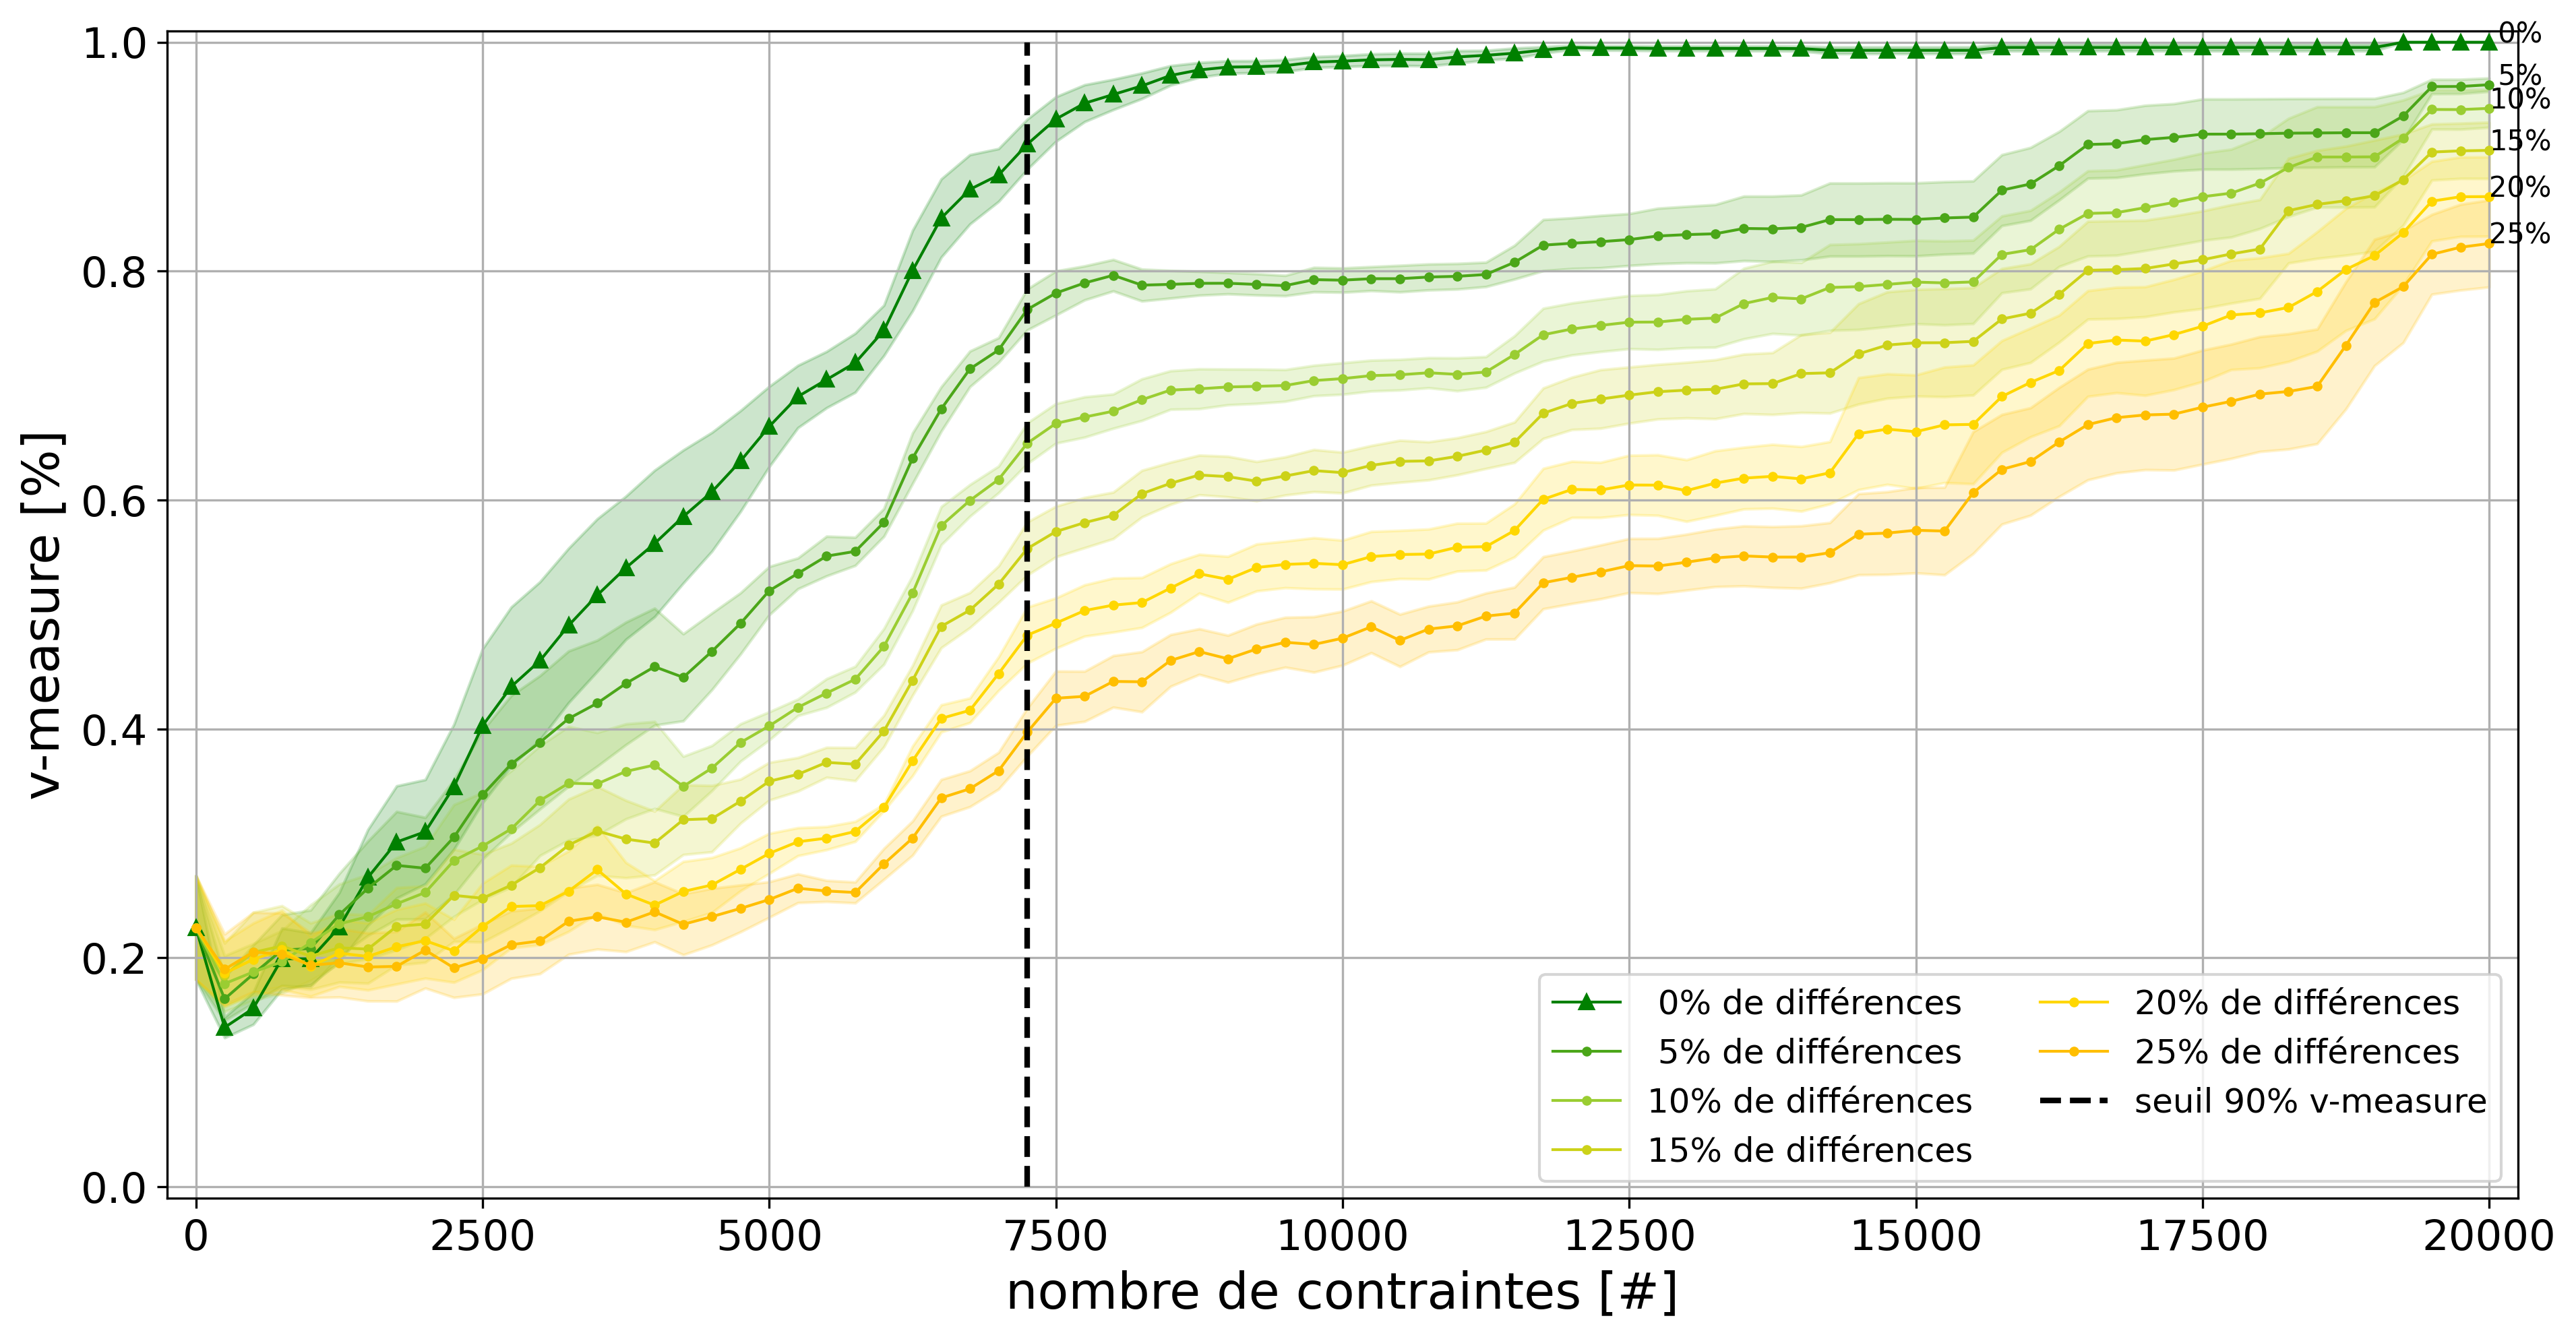
\includegraphics[width=0.95\textwidth]{figures/etude-erreur-simulation-impact-size-2000}
				\caption{
					Exemple d'une évolution de similitudes moyennes (calculées en terme de \texttt{v-measure}) de résultats de \textit{clustering} de tentatives introduisant des incohérences d'annotation par rapport à la vérité terrain au cours des itérations, exemple pour une vérité terrain ayant une taille de $2~000$ données.
					Les dégradés de couleurs des courbes représentent les déclinaisons de ces évolutions en fonction des différents taux d'annotations erronées (allant de $0$\% et $25$\%).
					La barre verticale indique le nombre de contraintes nécessaires aux tentatives n'introduisant pas d'incohérences pour obtenir une moyenne de $90$\% de \texttt{v-measure} (ici: $7~250$).
				}
				\label{figure:4.6.2-ETUDE-ROBUSTESSE-SIMULATION-IMPACT-DIFFERENCES-2000}
			\end{figure}
			
			% % Table écart de performances.
			% \begin{table}[!htb]
				\small
				\footnotesize
				% \begin{center}
				% \scalebox{0.8}{
					% \begin{tabular}{|c|c|r|r|r|r|r|r|r|r|r|}
					
						% \hhline{~~|---------}
						% % ENTETE DU TABLEAU
						% \multicolumn{2}{c|}{}
							% & \multicolumn{9}{c|}{
								% \cellcolor{colorTableHeader!15}
								% \shortstack{Taille des jeux de données}
							% }
							% \tabularnewline
							% \hhline{~~|-|-|-|-|-|-|-|-|-|}
						% % Taille du jeu de données
						% \multicolumn{2}{c|}{}
							% & \cellcolor{colorTableHeader!15} $1~000$
							% & \cellcolor{colorTableHeader!15} $1~500$
							% & \cellcolor{colorTableHeader!15} $2~000$
							% & \cellcolor{colorTableHeader!15} $2~500$
							% & \cellcolor{colorTableHeader!15} $3~000$
							% & \cellcolor{colorTableHeader!15} $3~500$
							% & \cellcolor{colorTableHeader!15} $4~000$
							% & \cellcolor{colorTableHeader!15} $4~500$
							% & \cellcolor{colorTableHeader!15} $5~000$
							% \tabularnewline
							% \hhline{~|----------}
							
						% % Contraintes annotées.
						% \multicolumn{1}{c|}{}
							% & \cellcolor{colorTableHeader!15} \textit{Contraintes}
							% & \multirow{2}{*}{$4~250$}
							% & \multirow{2}{*}{$6~000$}
							% & \multirow{2}{*}{$7~250$}
							% & \multirow{2}{*}{$8~750$}
							% & \multirow{2}{*}{$10~250$}
							% & \multirow{2}{*}{$11~250$}
							% & \multirow{2}{*}{$12~250$}
							% & \multirow{2}{*}{$13~500$}
							% & \multirow{2}{*}{$16~250$}
							% \tabularnewline
						% \multicolumn{1}{c|}{}
							% & \cellcolor{colorTableHeader!15} \textit{annotées}
							% &
							% &
							% &
							% &
							% &
							% &
							% &
							% &
							% &
							% \tabularnewline
							% \hline
							
						% % Erreur 0%
						% \cellcolor{colorTableHeader!15}
							% & \cellcolor{colorTableHeader!15}
							% & $91.15$\%
							% & $91.95$\%
							% & $91.08$\%
							% & $92.60$\%
							% & $93.04$\%
							% & $90.25$\%
							% & $90.00$\%
							% & $90.18$\%
							% & $91.17$\%
							% \tabularnewline
						% \cellcolor{colorTableHeader!15}
							% & \multirow{-2}{*}{
								% \cellcolor{colorTableHeader!15}
								% $0$\%
							% }
							% & \footnotesize $(\pm3.04)$
							% & \footnotesize $(\pm2.68)$
							% & \footnotesize $(\pm2.19)$
							% & \footnotesize $(\pm1.23)$
							% & \footnotesize $(\pm1.51)$
							% & \footnotesize $(\pm3.22)$
							% & \footnotesize $(\pm2.47)$
							% & \footnotesize $(\pm2.60)$
							% & \footnotesize $(\pm2.03)$
							% \tabularnewline
							% \hhline{~----------}
							
						% % Erreur 0.05%
						% \cellcolor{colorTableHeader!15}
							% & \cellcolor{colorTableHeader!15}
							% & $83.55$\%
							% & $75.65$\%
							% & $76.65$\%
							% & $73.09$\%
							% & $73.04$\%
							% & $72.91$\%
							% & $70.33$\%
							% & $67.44$\%
							% & $69.57$\%
							% \tabularnewline
						% \cellcolor{colorTableHeader!15}
							% & \multirow{-2}{*}{
								% \cellcolor{colorTableHeader!15}
								% $5$\%
							% }
							% & \footnotesize $(\pm4.64)$
							% & \footnotesize $(\pm2.25)$
							% & \footnotesize $(\pm1.79)$
							% & \footnotesize $(\pm1.26)$
							% & \footnotesize $(\pm1.17)$
							% & \footnotesize $(\pm2.23)$
							% & \footnotesize $(\pm1.39)$
							% & \footnotesize $(\pm1.25)$
							% & \footnotesize $(\pm2.99)$
							% \tabularnewline
							% \hhline{~----------}
						
						% % Erreur 0.10%
						% \cellcolor{colorTableHeader!15}
							% & \cellcolor{colorTableHeader!15}
							% & $78.39$\%
							% & $64.96$\%
							% & $64.96$\%
							% & $60.62$\%
							% & $60.26$\%
							% & $60.53$\%
							% & $56.91$\%
							% & $52.54$\%
							% & $56.35$\%
							% \tabularnewline
						% \cellcolor{colorTableHeader!15}
							% & \multirow{-2}{*}{
								% \cellcolor{colorTableHeader!15}
								% $10$\%
							% }
							% & \footnotesize $(\pm7.04)$
							% & \footnotesize $(\pm2.21)$
							% & \footnotesize $(\pm1.78)$
							% & \footnotesize $(\pm1.36)$
							% & \footnotesize $(\pm1.14)$
							% & \footnotesize $(\pm2.10)$
							% & \footnotesize $(\pm1.42)$
							% & \footnotesize $(\pm1.34)$
							% & \footnotesize $(\pm3.33)$
							% \tabularnewline
							% \hhline{~----------}
						
						% % Erreur 0.15%
						% \cellcolor{colorTableHeader!15}
							% & \cellcolor{colorTableHeader!15}
							% & $73.16$\%
							% & $57.55$\%
							% & $55.76$\%
							% & $50.85$\%
							% & $47.42$\%
							% & $51.50$\%
							% & $48.08$\%
							% & $41.03$\%
							% & $46.94$\%
							% \tabularnewline
						% \cellcolor{colorTableHeader!15}
							% & \multirow{-2}{*}{
								% \cellcolor{colorTableHeader!15}
								% $15$\%
							% }
							% & \footnotesize $(\pm9.06)$
							% & \footnotesize $(\pm2.40)$
							% & \footnotesize $(\pm2.32)$
							% & \footnotesize $(\pm1.28)$
							% & \footnotesize $(\pm1.99)$
							% & \footnotesize $(\pm2.21)$
							% & \footnotesize $(\pm1.77)$
							% & \footnotesize $(\pm1.02)$
							% & \footnotesize $(\pm3.04)$
							% \tabularnewline
							% \hhline{~----------}
						
						% % Erreur 0.20%
						% \cellcolor{colorTableHeader!15}
							% & \cellcolor{colorTableHeader!15}
							% & $68.87$\%
							% & $51.17$\%
							% & $48.19$\%
							% & $41.46$\%
							% & $40.52$\%
							% & $43.03$\%
							% & $40.11$\%
							% & $34.07$\%
							% & $38.72$\%
							% \tabularnewline
						% \cellcolor{colorTableHeader!15}
							% & \multirow{-2}{*}{
								% \cellcolor{colorTableHeader!15}
								% $20$\%
							% }
							% & \footnotesize $(\pm9.93)$
							% & \footnotesize $(\pm2.37)$
							% & \footnotesize $(\pm2.45)$
							% & \footnotesize $(\pm0.98)$
							% & \footnotesize $(\pm1.92)$
							% & \footnotesize $(\pm1.76)$
							% & \footnotesize $(\pm2.04)$
							% & \footnotesize $(\pm0.90)$
							% & \footnotesize $(\pm2.31)$
							% \tabularnewline
							% \hhline{~----------}
						
						% % Erreur 0.25%
						% \cellcolor{colorTableHeader!15}
							% & \cellcolor{colorTableHeader!15}
							% & $64.63$\%
							% & $43.52$\%
							% & $39.72$\%
							% & $35.85$\%
							% & $34.67$\%
							% & $36.97$\%
							% & $32.22$\%
							% & $25.82$\%
							% & $31.38$\%
							% \tabularnewline
						% \multirow{-12}{*}{
							% \cellcolor{colorTableHeader!15}
							% \rotatebox[origin=c]{90}{Taux de différences simulées}
						% }
							% & \multirow{-2}{*}{
								% \cellcolor{colorTableHeader!15}
								% $25$\%
							% }
							% & \footnotesize $(\pm11.22)$
							% & \footnotesize $(\pm2.24)$
							% & \footnotesize $(\pm2.10)$
							% & \footnotesize $(\pm0.96)$
							% & \footnotesize $(\pm1.14)$
							% & \footnotesize $(\pm2.11)$
							% & \footnotesize $(\pm1.52)$
							% & \footnotesize $(\pm1.26)$
							% & \footnotesize $(\pm2.46)$
							% \tabularnewline
							% \hline
						
					% \end{tabular}
				% }
				% \end{center}
				% \caption{
					% Estimation de la \textbf{similitude moyenne} (calculée en terme de \texttt{v-measure}) des résultats de \textit{clustering} des tentatives introduisant des incohérences d'annotation \textbf{par rapport à la vérité terrain}.
					% Cette similitude est rapportée en fonction de la taille du jeu de données utilisé et du taux de contraintes divergentes introduites lors des tentatives.
					% Pour chaque taille de jeu de données, les calculs sont réalisés avec un nombre de contraintes fixe, choisi comme étant le nombre de contraintes nécessaires pour que les tentatives sans incohérences atteignent une \texttt{v-measure} moyenne de $90$\% avec la vérité terrain (ce nombre est rapporté en deuxième ligne).
				% }
				% \label{table:4.6.2-ETUDE-ROBUSTESSE-SIMULATION-IMPACT-DIFFERENCES-PERFORMANCES}
			% \end{table}
			%
			% % Analyse du tableau de performance: chute drastique de performance.
			% Nous pouvons constater les points suivants :
			% \begin{itemize}
				Taille fixe.
				% \item à taille de jeu de données fixe, le taux de performance diminue lorsque le taux d'incohérences introduites augmentent ;
				% l'amplitude de diminution moyenne varie entre $27$ points (pour une taille de $1~000$ données) et $64$ points (pour une taille de $4~500$ données).
				Taux fixe.
				% \item à un taux fixe d'incohérences introduites, le taux de performance diminue lorsque la taille du jeu de données augmentent ;
				% l'amplitude de diminution moyenne varie entre $14$ points (pour l'introduction de $25$\% d'incohérences) et $33$ points (pour l'introduction de $25$\% d'incohérences).
			% \end{itemize}
			% Nous pouvons en déduire que l'insertion de différences d'annotations impacte plus fortement les gros jeux de données.
			
			
			% Analyse de la figure et lien vers la table.
			Grâce à cette figure, on peut estimer à $7~250$ le nombre moyen de contraintes nécessaires à une tentative n'introduisant pas d'incohérence pour atteindre $90$\% de \texttt{v-measure} par rapport à la vérité terrain (celle ayant $2~000$ données).
			Sur cette base, nous pouvons identifier la similitude moyenne des résultats \textit{clustering} entre les tentatives introduisant des d'incohérences par rapport à leur tentatives associées n'en introduisant pas, calculée pour un nombre fixe de $7~250$ contraintes\footnote{
				Observation de $7~250$ contraintes nécessaires : lors d'une analyse théorique utilisant l'\textsc{Équation~\ref{equation:4.3.3-ETUDE-COUT-NOMBRE-CONTRAINTES}}, nous aurions estimé une moyenne de $6~300$ contraintes, ce qui aurait introduit une légère variation dans nos résultats.
			} et pour les $5$ simulations de différences d'annotation (ayant des taux entre $5$\% et $25$\%).
			Ces similitudes sont rapportées dans la \textsc{Table~\ref{table:4.6.2-ETUDE-ROBUSTESSE-SIMULATION-IMPACT-DIFFERENCES-CLUSTERING}}, chaque analyse sur une taille de jeu de données étant retranscrite dans une colonne dédiée.
			
			% Analyse du tableau de performance: chute drastique de performance.
			Nous pouvons constater les points suivants :
			\begin{itemize}
				% Taille fixe.
				\item à taille de jeu de données fixe, le taux de similitude diminue lorsque le taux d'incohérences introduites augmentent ;
				l'amplitude de diminution varie environ entre $33$ points (pour une taille de $1~000$ données) et $70$ points (pour une taille de $4~500$ données).
				% Taux fixe.
				\item à un taux fixe d'incohérences introduites, le taux de similitude diminue lorsque la taille du jeu de données augmentent ;
				l'amplitude de diminution varie environ entre $16$ points (pour l'introduction de $25$\% d'incohérences) et $34$ points (pour l'introduction de $25$\% d'incohérences).
			\end{itemize}
			
			% Table similitude avec clustering sans erreurs.
			\begin{table}[!htb]
				% \small
				% \footnotesize
				\begin{center}
				\scalebox{0.8}{
					\begin{tabular}{|c|c|r|r|r|r|r|r|r|r|r|}
					
						\hhline{~~|---------}
						% ENTETE DU TABLEAU
						\multicolumn{2}{c|}{}
							& \multicolumn{9}{c|}{
								\cellcolor{colorTableHeader!15}
								\shortstack{Taille des jeux de données}
							}
							\tabularnewline
							\hhline{~~|-|-|-|-|-|-|-|-|-|}
						% Taille du jeu de données
						\multicolumn{2}{c|}{}
							& \cellcolor{colorTableHeader!15} $1~000$
							& \cellcolor{colorTableHeader!15} $1~500$
							& \cellcolor{colorTableHeader!15} $2~000$
							& \cellcolor{colorTableHeader!15} $2~500$
							& \cellcolor{colorTableHeader!15} $3~000$
							& \cellcolor{colorTableHeader!15} $3~500$
							& \cellcolor{colorTableHeader!15} $4~000$
							& \cellcolor{colorTableHeader!15} $4~500$
							& \cellcolor{colorTableHeader!15} $5~000$
							\tabularnewline
							\hhline{~|----------}
							
						% Contraintes annotées.
						\multicolumn{1}{c|}{}
							& \cellcolor{colorTableHeader!15} \textit{Contraintes}
							& \multirow{2}{*}{$4~250$}
							& \multirow{2}{*}{$6~000$}
							& \multirow{2}{*}{$7~250$}
							& \multirow{2}{*}{$8~750$}
							& \multirow{2}{*}{$10~250$}
							& \multirow{2}{*}{$11~250$}
							& \multirow{2}{*}{$12~250$}
							& \multirow{2}{*}{$13~500$}
							& \multirow{2}{*}{$16~250$}
							\tabularnewline
						\multicolumn{1}{c|}{}
							& \cellcolor{colorTableHeader!15} \textit{annotées}
							&
							&
							&
							&
							&
							&
							&
							&
							&
							\tabularnewline
							\hline
							
						% Erreur 0%
						\cellcolor{colorTableHeader!15}
							& \cellcolor{colorTableHeader!15}
							& $97.46$\%
							& $96.17$\%
							& $95.03$\%
							& $95.58$\%
							& $95.42$\%
							& $94.75$\%
							& $94.74$\%
							& $96.00$\%
							& $93.15$\%
							\tabularnewline
						\cellcolor{colorTableHeader!15}
							& \multirow{-2}{*}{
								\cellcolor{colorTableHeader!15}
								$0$\%
							}
							& \footnotesize $(\pm0.65)$
							& \footnotesize $(\pm0.99)$
							& \footnotesize $(\pm1.08)$
							& \footnotesize $(\pm0.79)$
							& \footnotesize $(\pm0.84)$
							& \footnotesize $(\pm1.43)$
							& \footnotesize $(\pm1.12)$
							& \footnotesize $(\pm0.78)$
							& \footnotesize $(\pm1.23)$
							\tabularnewline
							\hhline{~----------}
							
						% Erreur 0.05%
						\cellcolor{colorTableHeader!15}
							& \cellcolor{colorTableHeader!15}
							& $85.10$\%
							& $76.76$\%
							& $77.85$\%
							& $73.50$\%
							& $73.34$\%
							& $73.50$\%
							& $70.74$\%
							& $68.97$\%
							& $68.72$\%
							\tabularnewline
						\cellcolor{colorTableHeader!15}
							& \multirow{-2}{*}{
								\cellcolor{colorTableHeader!15}
								$5$\%
							}
							& \footnotesize $(\pm1.85)$
							& \footnotesize $(\pm0.95)$
							& \footnotesize $(\pm0.78)$
							& \footnotesize $(\pm0.81)$
							& \footnotesize $(\pm0.57)$
							& \footnotesize $(\pm1.01)$
							& \footnotesize $(\pm0.47)$
							& \footnotesize $(\pm0.58)$
							& \footnotesize $(\pm1.31)$
							\tabularnewline
							\hhline{~----------}
						
						% Erreur 0.10%
						\cellcolor{colorTableHeader!15}
							& \cellcolor{colorTableHeader!15}
							& $79.29$\%
							& $65.03$\%
							& $65.46$\%
							& $60.45$\%
							& $60.59$\%
							& $60.32$\%
							& $57.15$\%
							& $53.34$\%
							& $55.55$\%
							\tabularnewline
						\cellcolor{colorTableHeader!15}
							& \multirow{-2}{*}{
								\cellcolor{colorTableHeader!15}
								$10$\%
							}
							& \footnotesize $(\pm3.06)$
							& \footnotesize $(\pm1.06)$
							& \footnotesize $(\pm0.78)$
							& \footnotesize $(\pm0.76)$
							& \footnotesize $(\pm0.51)$
							& \footnotesize $(\pm0.99)$
							& \footnotesize $(\pm0.68)$
							& \footnotesize $(\pm0.84)$
							& \footnotesize $(\pm1.50)$
							\tabularnewline
							\hhline{~----------}
						
						% Erreur 0.15%
						\cellcolor{colorTableHeader!15}
							& \cellcolor{colorTableHeader!15}
							& $73.67$\%
							& $57.84$\%
							& $56.21$\%
							& $50.50$\%
							& $47.56$\%
							& $51.65$\%
							& $48.16$\%
							& $41.68$\%
							& $46.29$\%
							\tabularnewline
						\cellcolor{colorTableHeader!15}
							& \multirow{-2}{*}{
								\cellcolor{colorTableHeader!15}
								$15$\%
							}
							& \footnotesize $(\pm4.08)$
							& \footnotesize $(\pm1.14)$
							& \footnotesize $(\pm0.97)$
							& \footnotesize $(\pm0.72)$
							& \footnotesize $(\pm0.98)$
							& \footnotesize $(\pm1.04)$
							& \footnotesize $(\pm0.74)$
							& \footnotesize $(\pm0.65)$
							& \footnotesize $(\pm1.37)$
							\tabularnewline
							\hhline{~----------}
						
						% Erreur 0.20%
						\cellcolor{colorTableHeader!15}
							& \cellcolor{colorTableHeader!15}
							& $68.86$\%
							& $51.28$\%
							& $48.21$\%
							& $41.58$\%
							& $40.99$\%
							& $43.00$\%
							& $40.18$\%
							& $34.41$\%
							& $38.37$\%
							\tabularnewline
						\cellcolor{colorTableHeader!15}
							& \multirow{-2}{*}{
								\cellcolor{colorTableHeader!15}
								$20$\%
							}
							& \footnotesize $(\pm4.59)$
							& \footnotesize $(\pm1.15)$
							& \footnotesize $(\pm1.10)$
							& \footnotesize $(\pm0.47)$
							& \footnotesize $(\pm0.94)$
							& \footnotesize $(\pm0.84)$
							& \footnotesize $(\pm0.90)$
							& \footnotesize $(\pm0.54)$
							& \footnotesize $(\pm1.05)$
							\tabularnewline
							\hhline{~----------}
						
						% Erreur 0.25%
						\cellcolor{colorTableHeader!15}
							& \cellcolor{colorTableHeader!15}
							& $64.89$\%
							& $43.63$\%
							& $39.60$\%
							& $35.70$\%
							& $34.94$\%
							& $37.00$\%
							& $32.12$\%
							& $26.49$\%
							& $31.24$\%
							\tabularnewline
						\multirow{-12}{*}{
							\cellcolor{colorTableHeader!15}
							\rotatebox[origin=c]{90}{Taux de différences simulées}
						}
							& \multirow{-2}{*}{
								\cellcolor{colorTableHeader!15}
								$25$\%
							}
							& \footnotesize $(\pm5.15)$
							& \footnotesize $(\pm1.12)$
							& \footnotesize $(\pm0.97)$
							& \footnotesize $(\pm0.47)$
							& \footnotesize $(\pm0.57)$
							& \footnotesize $(\pm0.99)$
							& \footnotesize $(\pm0.70)$
							& \footnotesize $(\pm0.72)$
							& \footnotesize $(\pm1.11)$
							\tabularnewline
							\hline
						
					\end{tabular}
				}
				\end{center}
				\caption{
					Estimation de la \textbf{similitude moyenne} (calculée en terme de \texttt{v-measure}) des résultats de \textit{clustering} des tentatives introduisant des incohérences d'annotation \textbf{par rapport aux résultats de \textit{clustering} des tentatives n'en introduisant pas}. \\
					Cette similitude est rapportée en fonction de la taille du jeu de données utilisé et du taux de contraintes divergentes introduites lors des tentatives.
					Pour chaque taille de jeu de données, les calculs sont réalisés avec un nombre de contraintes fixe, choisi comme étant le nombre de contraintes nécessaires pour que les tentatives sans incohérences atteignent une \texttt{v-measure} moyenne de $90$\% avec la vérité terrain (ce nombre est rapporté en deuxième ligne).
				}
				\label{table:4.6.2-ETUDE-ROBUSTESSE-SIMULATION-IMPACT-DIFFERENCES-CLUSTERING}
			\end{table}

		%%% Discussion
		\subsubsection{Discussion}
		
			% Rappel de l'objectif : ...
			\todo[inline]{A REDIGER: rappel de l'objectif}
		
			% Remaques expérience utilisateur.
			\todo[inline]{A REDIGER: rappel: les clustering erronés divergent de la vérité terrain}
			\todo[inline]{A REDIGER: les clustering sein et erronés divergent aussi !}
			\todo[inline]{A REDIGER: cette divergence est plus forte si les visions/complexité est plus grande, mais aussi si le jeu de données est plus grand (normal, il y a moins de redondance et plus de change de diverger}
			
			% Conclusions et suggestion.
			\todo[inline]{A REDIGER: vraiment important de mettre plus de monde dessus}
			
			
	%%%
	%%% Subsection 4.6.3: Étude du score inter-annotateurs obtenu avec des opérateurs en situation réelle.
	%%%
	\subsection{Étude du score inter-annotateurs obtenu avec des opérateurs en situation réelle}
	\label{section:4.6.3-ETUDE-ROBUSTESSE-SCORE-INTER-ANNOTATEURS}
		
		% Objectif de l'expérience.
		Pour terminer, nous voulons étudier le score d'accord inter-annotateurs calculé lors d'une annotation de contraintes par plusieurs experts métiers en situation réelle.
		Pour cela, nous reprenons l'expérience de la \textsc{Section~\ref{section:4.3.1-ETUDE-COUTS-TEMPS-ANNOTATION}} visant à estimer le temps moyen d'annotation d'un lot de contraintes, et nous réutilisons ses résultats pour en estimer l'accord inter-annotateurs.
		Comme l'objectif n'était pas d'étudier la qualité des annotation, aucun guide ni aucune règles d'annotation précises n'avaient été fournies.
		Nous espérons donc pourvoir estimer une borne maximale grossière de l'accord inter-annotateurs de notre méthode sans concertation.
		
		%%% Protocole expérimental.
		\subsubsection{Protocole expérimental}
			
			% Axiome.
			\begin{leftBarWarning}
				Pour l'étude d'annotation en \textsc{Section~\ref{section:4.3.1-ETUDE-COUTS-TEMPS-ANNOTATION}}, nous avions supposons que les annotateurs de l'expérience connaissaient parfaitement le domaine traité dans le jeu de données, et qu'ils sont capables de caractériser sans ambiguïté la similitude entre deux données issues de cet ensemble.
				Afin de pourvoir faire cette hypothèse forte, et ainsi limiter les bruits dans l'analyse des résultats, le jeu de données choisi devait traiter d'un sujet de culture générale (ne nécessitant donc pas de connaissance particulière) et des réviseurs avaient supprimer en amont et d'un commun accord les données trop spécifiques ou trop ambiguës.
			\end{leftBarWarning}
			
			% Pseudo-code.
			Pour résumer le protocole expérimental que nous décrivons ci-dessous, vous pouvez vous référer au pseudo-code décrit dans \textsc{Algorithme~\ref{algorithm:4.6.3-ETUDE-ROBUSTESSE-SCORE-INTER-ANNOTATEURS-PROTOCOLE}}.

			\begin{algorithm}
				\KwData{jeu de données annotées (vérité terrain)}
				\KwIn{plusieurs réviseurs, plusieurs annotateurs}
				%
				\textbf{initialisation}: définir et revoir le jeu de données entre réviseurs \;
				\textbf{échantillonnage}: sélectionner une base de contraintes équilibrée \;
				\ForEach{annotateur}{
					 \While{la base de contraintes n'a pas été entièrement annotée}{
						\textbf{annotation}: annoter une partie des contraintes \;
						\textbf{revue}: revue des contraintes en conflits d'annotation \;
					}
				}
				%
				\KwResult{modélisation du score inter-annotateurs sur le lot de contraintes}
				%
				\caption{\textit{
					Description en pseudo-code du protocole expérimental de l'étude du score inter-annotateurs d'annotation d'un lot de contraintes par plusieurs experts métiers en situation réelle.
				}}
				\label{algorithm:4.6.3-ETUDE-ROBUSTESSE-SCORE-INTER-ANNOTATEURS-PROTOCOLE}
			\end{algorithm}
			
			% Détails de l'expérience : préparation du jeu de données.
			Concernant la précédente expérience d'annotation en situation réelle, nous avions procédé en plusieurs étapes.
			D'abord, il fallait choisir un jeu de données approprié : pour valider notre hypothèse forte sur les compétences de nos annotateurs, nous cherchions un jeu de données traitant d'un sujet de culture général.
			Pour cette expérience, nous avions donc choisi \texttt{MLSUM} : une collecte d'articles de journaux, classés par catégorie de publication et décrits par leur titre et leur résumé.
			Nous nous intéressions ici à la tâche de classification d'un titre d'article en fonction de sa catégorie de publication.
			Comme certains titres pouvaient porter à confusion (un titre d'article n'étant pas toujours explicite sur son contenu), deux réviseurs furent chargés de choisir les données les plus explicites sur un échantillon d'un millier de données représentatives des catégories les plus communes.
			L'échantillon résultant, noté \texttt{MLSUM FR Train Subset (v1.0.0-schild)}, est composé de $744$ titres d'articles rédigés en français et répartis en $14$ classes (\textit{économie}, \textit{sport}, ...).
			Pour plus de détails, consultez l'annexe~\ref{annex:A.2-DATASET-MLSUM-SUBSET-SCHILD}.
		
			% Détails de l'expérience : sélection des contraintes à annoter.
			À partir de ces données, nous avions sélectionné un lot de $400$ contraintes à annoter.
			Pour faciliter l'analyse, l'échantillonnage fut un aléatoire équilibré d'après la vérité terrain en $200$ \texttt{MUST-LINK} et en $200$ \texttt{CANNOT-LINK}.
			
			% Détails de l'expérience : annotations et consignes.
			Ensuite, un groupe de $3$ annotateurs ont annoté la sélection de $400$ contraintes en plusieurs sessions.
			Les directives données aux opérateurs étaient les suivantes:
			\begin{itemize}
				\item \textbf{Contexte de l'opérateur} :
				\textguillemets{\textit{Vous êtes des \textbf{experts de la presse et de l’actualité} ; Vous voulez classer des articles dans des catégories en fonction de leur titre ; Vous ne savez pas précisément quelles catégories vous allez utiliser pour classer vos articles ; Mais vous savez \textbf{caractériser la similitude} de deux articles}} ;
				\item \textbf{Contexte sur le jeu de données} :
				\textguillemets{\textit{Le thème sont les catégories d’articles de presse ; La vérité terrain contient entre $10$ et $20$ catégories parmi les plus communes de la presse ; La vérité terrain contient entre $30$ et $100$ articles par catégorie ; Vous \textbf{pouvez regarder le jeu de données non annoté} autant que vous le voulez (disponible dans l'onglet \texttt{TEXTS} de l'application)}} ;
				\item \textbf{Consignes d'annotations} :
				\textguillemets{\textit{Faites des séries de \textbf{15 minutes minimum} pour avoir de la régularité ; Si possible, \textbf{isolez-vous} pour ne pas être dérangé et ne pas fausser les résultats ; Pour chaque série, \textbf{notez le temps et le nombre de contraintes annotés} ; Si vous ne savez pas quoi annoter (trop ambigu, vocabulaire inconnu, ...), \textbf{passez au suivant sans annoter} (vous êtes sensés être des experts de la presse !)}}.
			\end{itemize}
			%
			Pour réaliser l'annotation, les opérateurs eurent accès à l'application web développée au cours de ce doctorat.
			Des captures d'écran sont disponibles en \textsc{Figure~\ref{figure:4.3.1-ETUDE-COUTS-TEMPS-ANNOTATION-APPLICATION-ANNOTATION}} et \textsc{Figure~\ref{figure:4.3.1-ETUDE-COUTS-TEMPS-ANNOTATION-APPLICATION-LISTE-CONTRAINTES}}.
			Une description plus détaillée de l'application et de ses fonctionnalités est disponible en \textsc{Section~\ref{section:3.3-DESCRIPTION-IMPLEMENTATION}}\todo{description à faire}.
			
			% Détails de l'expérience.
			Pour cette étude, nous allons réutiliser ces annotations et calculé le score d'accord inter-annotateur global et deux à deux.
			Pour ce faire, nous allons utiliser l'$\alpha$ de \textit{Krippendorff} (\cite{krippendorff:2004:content-analysis-introduction}) implémenté dans la librairie \texttt{simpledorff} (\cite{perry:2021:lighttag-text-annotation}).
			
			% Référence scripts.
			\begin{leftBarInformation}
				Les scripts de l'expérience, réalisés avec des \textit{notebooks} Python (\cite{van-rossum-drake:2009:python-reference-manual}), sont disponibles dans un dossier dédié de~\cite{schild:2021:cognitivefactory-interactiveclusteringcomparativestudy}.
			\end{leftBarInformation}
			
		%%% Résultats
		\subsubsection{Résultats obtenus}
		
			% Description statistiques.
			La \textsc{Table~\ref{table:4.6.3-ETUDE-ROBUSTESSE-SCORE-INTER-ANNOTATEURS}} expose les scores inter-annotateurs sur les $3$ opérateurs et le réviseur de cette expérience, ainsi que l'accord avec la vérité terrain.
			Le score d'accord moyen avec la vérité terrain est de $0.86$ (écart-type: $0.01$) ; ce score est de $0.81$ (écart-type: $0.05$) pour les contraintes de types \texttt{MUST-LINK} et est de $0.92$ (écart-type: $0.03$) pour les contraintes de types \texttt{CANNOT-LINK}.
			Le score inter-annotateurs moyen (sans le réviseur) est de $0.84$ (écart-type: $0.03$).
			
			\begin{table}[!htb]
				\begin{center}
				\begin{tabular}{|c|r|r|r|r|}
				
					\hline
					% ENTETE DU TABLEAU
					\rowcolor{colorTableHeader!15}
					
						& \multicolumn{1}{c|}{\shortstack[c]{
							1 (Relecteur)
						}}
						& \multicolumn{1}{c|}{\shortstack[c]{
							7 (Annotateur)
						}}
						& \multicolumn{1}{c|}{\shortstack[c]{
							9 (Annotateur)
						}}
						& \multicolumn{1}{c|}{\shortstack[c]{
							12 (Annotateur)
						}}
						\tabularnewline
						\hline

					% Vérité terrain
					\multicolumn{1}{|c|}{\shortstack[c]{
						Vérité terrain
					}}
						& $0.95$
						& $0.86$
						& $0.84$
						& $0.87$
						\tabularnewline
						\hline

					% Vérité terrain
					\multicolumn{1}{|c|}{\shortstack[c]{
						1 (Relecteur)
					}}
						&
						& $0.91$
						& $0.86$
						& $0.89$
						\tabularnewline
						\hline

					% Vérité terrain
					\multicolumn{1}{|c|}{\shortstack[c]{
						7 (Annotateur)
					}}
						&
						&
						& $0.86$
						& $0.85$
						\tabularnewline
						\hline

					% Vérité terrain
					\multicolumn{1}{|c|}{\shortstack[c]{
						9 (Annotateur)
					}}
						&
						&
						&
						& $0.80$
						\tabularnewline
						\hline
					
				\end{tabular}
				\end{center}
				\caption{
					Score d'accord inter-annotateurs obtenu avec $1$ réviseur et $3$ annotateurs sur un lot commun de $400$ contraintes ($200$ \texttt{MUST-LINK}, $200$ \texttt{CANNOT-LINK}).
				}
				\label{table:4.6.3-ETUDE-ROBUSTESSE-SCORE-INTER-ANNOTATEURS}
			\end{table}
			
			% Note.
			\begin{leftBarInformation}
				Dans une autre expérience, où $14$ opérateurs devaient annoter une base de $1~000$ contraintes aléatoires, nous obtenons un accord moyen avec la vérité terrain de $0.93$ (écart-type: $0.02$) et un score inter-annotateurs moyen de $0.91$ (écart-type: $0.03$).
				Toutefois, nous ne mettons pas en avant ces résultats car le lot de contraintes à annoté est déséquilibré à cause de l'utilisation de l'échantillonnage aléatoire ($932$ \texttt{CANNOT-LINK}, $68$ \texttt{MUST-LINK}).
			\end{leftBarInformation}
	
		%%% Discussion
		\subsubsection{Discussion}
		
			% Rappel de l'objectif : ...
			\todo[inline]{A REDIGER: rappel de l'objectif}
		
			% Avantage 1 : peu d'erreurs
			\todo[inline]{A REDIGER: Peu d'erreurs (environ 16\% d'erreurs sans concertations)}
			
			% Remarque 1 : MUST-LINK < CANNOT-LINK
			\todo[inline]{A REDIGER: CANNOT-LINK légèrement plus facile que les MUST-LINK}
			
			% Conclusions et suggestion.
			\todo[inline]{A REDIGER: ouverture sur l'impact des non-corrections}
			
	%%%
	%%% Subsection 4.6.3: Bilan concernant la robustesse du \textit{clustering} interactif
	%%%
	\subsection{Bilan concernant la robustesse du \textit{clustering} interactif}
	\label{section:4.6.3-ETUDE-ROBUSTESSE-MISE-EN-COMMUN}
	
		\todo[inline]{A REDIGER}
	
		% Conclusion.
		\begin{leftBarSummary}
			Au cours de cette étude de pertinence, nous avons pu voir que :
			\begin{itemize}
				\item[\itemok] ...
				\item[\itemok] ...
				\item[\itemok] ...
			\end{itemize}
		\end{leftBarSummary}